% (C) Marc Lijour, 2018 
% Licensed under a Creative Commons License BY-SA
% https://creativecommons.org/licenses/by-sa/2.5/ca/
% Technical Workshop for BlockHack , given April 21, 2018
% Introduction to Blockchain/Decentralized Application Development
% A primer on Ethereum, on the ConsenSys stack
% 
% Variables
% TODO set the variables
% ---------------------- USER-DEFINED --------------------------------
\newcommand{\ConsenSystitle}{ConsenSys}
\newcommand{\ConsenSyslongtitle}{Intro to Ethereum Development and ConsenSys tools}
\newcommand{\ConsenSyssubtitle}{A primer}
\newcommand{\ConsenSysauthor}{Marc~Lijour}
\newcommand{\ConsenSysdate}{April 21, 2018}
\newcommand{\ConsenSyssubject}{ConsenSys}
% --------------------------------------------------------------------
% Template
% (C) Marc Lijour, 2018
% (C) ConsenSys for logos, trademarked materials
% This document is licensed under a Creative Commons License BY-SA (feel free to use the code, but all rights are reserved for logos and art)
% https://creativecommons.org/licenses/by-sa/2.5/ca/
% ConsenSys presentation template in LaTeX
% This template comes with a first page on a picture background
% Possible improvement in future iterations
% - Test and fix as needed to work on xetex (to use Ubuntu fonts)
% === USAGE===
% Create a file for your LaTeX content (slides, etc), in which you must do the following:
% TODO 1 - set variables defined below
% TODO 2 - include this code by calling: \input{<the name of this document>}
% TODO 3 - Start the document as usual and you're in business; just use \begin{document} and don't forget to conclude with \end{document}
% TODO 4 - Use the custom method \ConsenSyscoverpage instead of \titlepage to create your cover page
% Voilà!
%
\documentclass[utf8]{beamer}
\usepackage{etoolbox}
%\usepackage[american,french]{babel}
%\usepackage[T1]{fontenc}
%\usepackage[utf8]{inputenc}
% Variables
% ---------------------- USER-DEFINED --------------------------------
\ifdef{\ConsenSystitle}{}{\newcommand{\ConsenSystitle}{\color{red}Title TBD}}
\ifdef{\ConsenSyslongtitle}{}{\newcommand{\ConsenSyslongtitle}{\color{red}Long title TBD}}
\ifdef{\ConsenSyssubtitle}{}{\newcommand{\ConsenSyssubtitle}{\color{red}Subtitle TBD}}
\ifdef{\ConsenSysauthor}{}{\newcommand{\ConsenSysauthor}{\color{red}Author TBD}}
\ifdef{\ConsenSysdate}{}{\newcommand{\ConsenSysdate}{\color{red}Date TBD}}
\ifdef{\ConsenSyssubject}{}{\newcommand{\ConsenSyssubject}{\color{red}Subject TBD}}
% --------------------------------------------------------------------
\usetheme{Boadilla}
% Set color close to ConsenSys paletter
%\definecolor{beamer@blendedblue}{RGB}{150,36,36}
\definecolor{beamer@blendedblue}{RGB}{47,57,118}
% Cover Page
\title[\ConsenSystitle] {\ConsenSyslongtitle}
\subtitle{\ConsenSyssubtitle}
\author{\ConsenSysauthor}
\date{\ConsenSysdate}
\subject{\ConsenSyssubject}
\usepackage{tikz}
% Try Xetex to use system fonts (pdflatex makes it hard to import a font)
%\usepackage{fontspec}
%\setsansfont{Ubuntu}
%\setmonofont{Ubuntu Mono}

% -- create a custom (command) title page -which has the benefit of not affecting the settings for the rest of the presentation
\newcommand{\ConsenSyscoverpage}{\frame[plain]{
	\tikz[remember picture,overlay] {
        	\node(bkgd) at ([xshift=0cm,yshift=0cm]current page.center) 
			{
\includegraphics[width=\paperwidth, height=\paperheight]{../../ConsenSys-LaTeX_Templates/images/bkg-plain}};
        	\node(logo) at ([xshift=0cm,yshift=2.7cm]current page.center) 
%		 	{
\includegraphics[scale=.6]{../../ConsenSys-LaTeX_Templates/images/logohorizontal-white-on-darkblue}};
		 	{
\includegraphics[scale=.1]{../../ConsenSys-LaTeX_Templates/images/ConsenSys-logo-horizontal-white.png}};
        	\node(CC-BY-SA) at ([xshift=5cm,yshift=-4cm]current page.center) 
			{\href{https://creativecommons.org/licenses/by-sa/2.5/ca/}{
\includegraphics[scale=.4]{../../ConsenSys-LaTeX_Templates/images/CC-BY-SA-403x141}}};
	}
	\tikz[remember picture,overlay] {
        	\node(title) at ([xshift=0cm,yshift=0cm]current page.center) 
			%{\Large\color{black}\textbf{{\ConsenSyslongtitle}}};
			%{\Large\color{beamer@blendedblue}\textbf{{\ConsenSyslongtitle}}};
			{\Large\color{white}\textbf{{\ConsenSyslongtitle}}};
        	\node(subtitle) at ([xshift=0cm,yshift=-.7cm]current page.center) 
			%{\small\color{beamer@blendedblue}\emph{\ConsenSyssubtitle}};
			{\small\color{white}\emph{\ConsenSyssubtitle}};
        	\node(author) at ([xshift=0cm,yshift=-2cm]current page.center) 
			%{\small\color{beamer@blendedblue}By~\ConsenSysauthor};
			{\small\color{white}By~\ConsenSysauthor};
        	\node(date) at ([xshift=0cm,yshift=-2.5cm]current page.center) 
			%{\tiny\color{beamer@blendedblue}\ConsenSysdate};
			{\tiny\color{white}\ConsenSysdate};
        	\node(footnote) at ([xshift=0cm,yshift=-3.9cm]current page.center) 
			%{\TINY\color{beamer@blendedblue}\emph{The Art and Science of Eternal Blossom}};
			{\TINY\color{white}\emph{One of the largest blockchain companies in the world with 1,000 employees in 30 countries}};
        	%\node(footnote) at ([xshift=0cm,yshift=-4.1cm]current page.center) 
		%	{\TINY\color{black}\emph{focusing on Blockchain and related technologies}};
    	}
}}
%
% This sets the ColliderX logo at the bottom right corner of each page
\logo{
	
\includegraphics[scale=.07]{../../ConsenSys-LaTeX_Templates/images/consensys-logo-noname-transparent}
}
\AtBeginSection[]
{
  \begin{frame}
    \frametitle{Table of Contents}
    \tableofcontents[currentsection]
  \end{frame}
}
%\usepackage{newunicodechar}
%\usepackage[format=plain,justification=raggedright,singlelinecheck=false]{caption}
\usepackage[format=plain,justification=justified,singlelinecheck=false]{caption} % use this in document to remove "figure": 
%	\captionsetup{labelformat=empty}\caption{caption content} 
% or
% 	\caption*{caption content here}
\usepackage{dirtytalk}
\usepackage{wrapfig}
\usepackage{hyperref}
\usepackage{verbatim}
\usepackage{mathabx}
%\usepackage{MnSymbol}
\usepackage{fancyvrb}


% Extra packages
\usepackage{amssymb}
\usepackage{amsmath}
\usepackage[american]{babel}
\usepackage{csquotes}
\usepackage[backend=biber,style=apa]{biblatex}
\DeclareLanguageMapping{american}{american-apa}
% Use one bib file per section
\addbibresource{references.bib}
\addbibresource{references-ethereum-history.bib}
\definecolor{links}{HTML}{2A1B81}
\hypersetup{colorlinks,linkcolor=,urlcolor=links}
\AtBeginBibliography{\footnotesize}
% Start of the document
\begin{document}
% Cover page
% Do not use this: \frame{\titlepage}
% use this instead:
\ConsenSyscoverpage

% Content
% (C) Marc Lijour, 2018 
% Licensed under a Creative Commons License BY-SA
% https://creativecommons.org/licenses/by-sa/2.5/ca/
% Presentation for Mexican students during TECinToronto, Starfield
% Hands-on Introduction to Blockchain
% 
\frame{
	\frametitle{Who am I?}
	\framesubtitle{\url{https://www.linkedin.com/in/marclijour/}}
	\begin{columns}
	\column{0.5\textwidth}
		\begin{figure}
		
\includegraphics[width=3cm]{../pics/logos/colliderx_logo}
		\end{figure}
	\column{0.5\textwidth}
		\begin{figure}
		
\includegraphics[width=5.5cm]{../pics/logos/consensys-logo-v-630x581}
		\end{figure}
	\end{columns}
}

\frame{
	\frametitle{Access these slides}
	\center\Huge 
	\url{https://bit.ly/2rvX2HJ}\\ 
	\vspace{2em}
	{\Large 
		or find by date:\\
		\url{https://github.com/marclijour/presentations}
	}
}


% ======================================================================================================
%                         Hands-on Introduction to Crypto, Wallets, and Custom Tokens 
% ======================================================================================================
\section{Hands-on Introduction to Crypto}
\frame{
	\frametitle{}
	\centering\Huge
	Let's try things out!
}

\frame{
	\frametitle{Install MetaMask}
	\begin{columns}
	\column{0.6\textwidth}
		Follow step by step:
		\begin{enumerate}
			\item Install the \href{https://chrome.google.com/webstore/detail/metamask/nkbihfbeogaeaoehlefnkodbefgpgknn}{Chrome/Chromium extension} 
			\item Watch the \href{https://www.youtube.com/watch?v=6Gf\_kRE4MJU}{intro on Youtube}
			\item Create an account 
			\item Switch to the Ropsten Testnet (top-right in MetaMask) 
			\item Fill your account with Ether from \url{https://faucet.metamask.io}
		\end{enumerate}
	\column{0.4\textwidth}
		\begin{figure}
			
\includegraphics[width=3cm]{../pics/ethereum/metamask-logo}
			\captionsetup{justification=centering}
			\caption*{\url{https://metamask.io}}
		\end{figure}
	\end{columns}
}

\frame{
	\frametitle{Request Ether from the faucet (on the Ropsten network)}
	\framesubtitle{Do it several times; then donate 1 ether to the faucet}
	\begin{figure}
		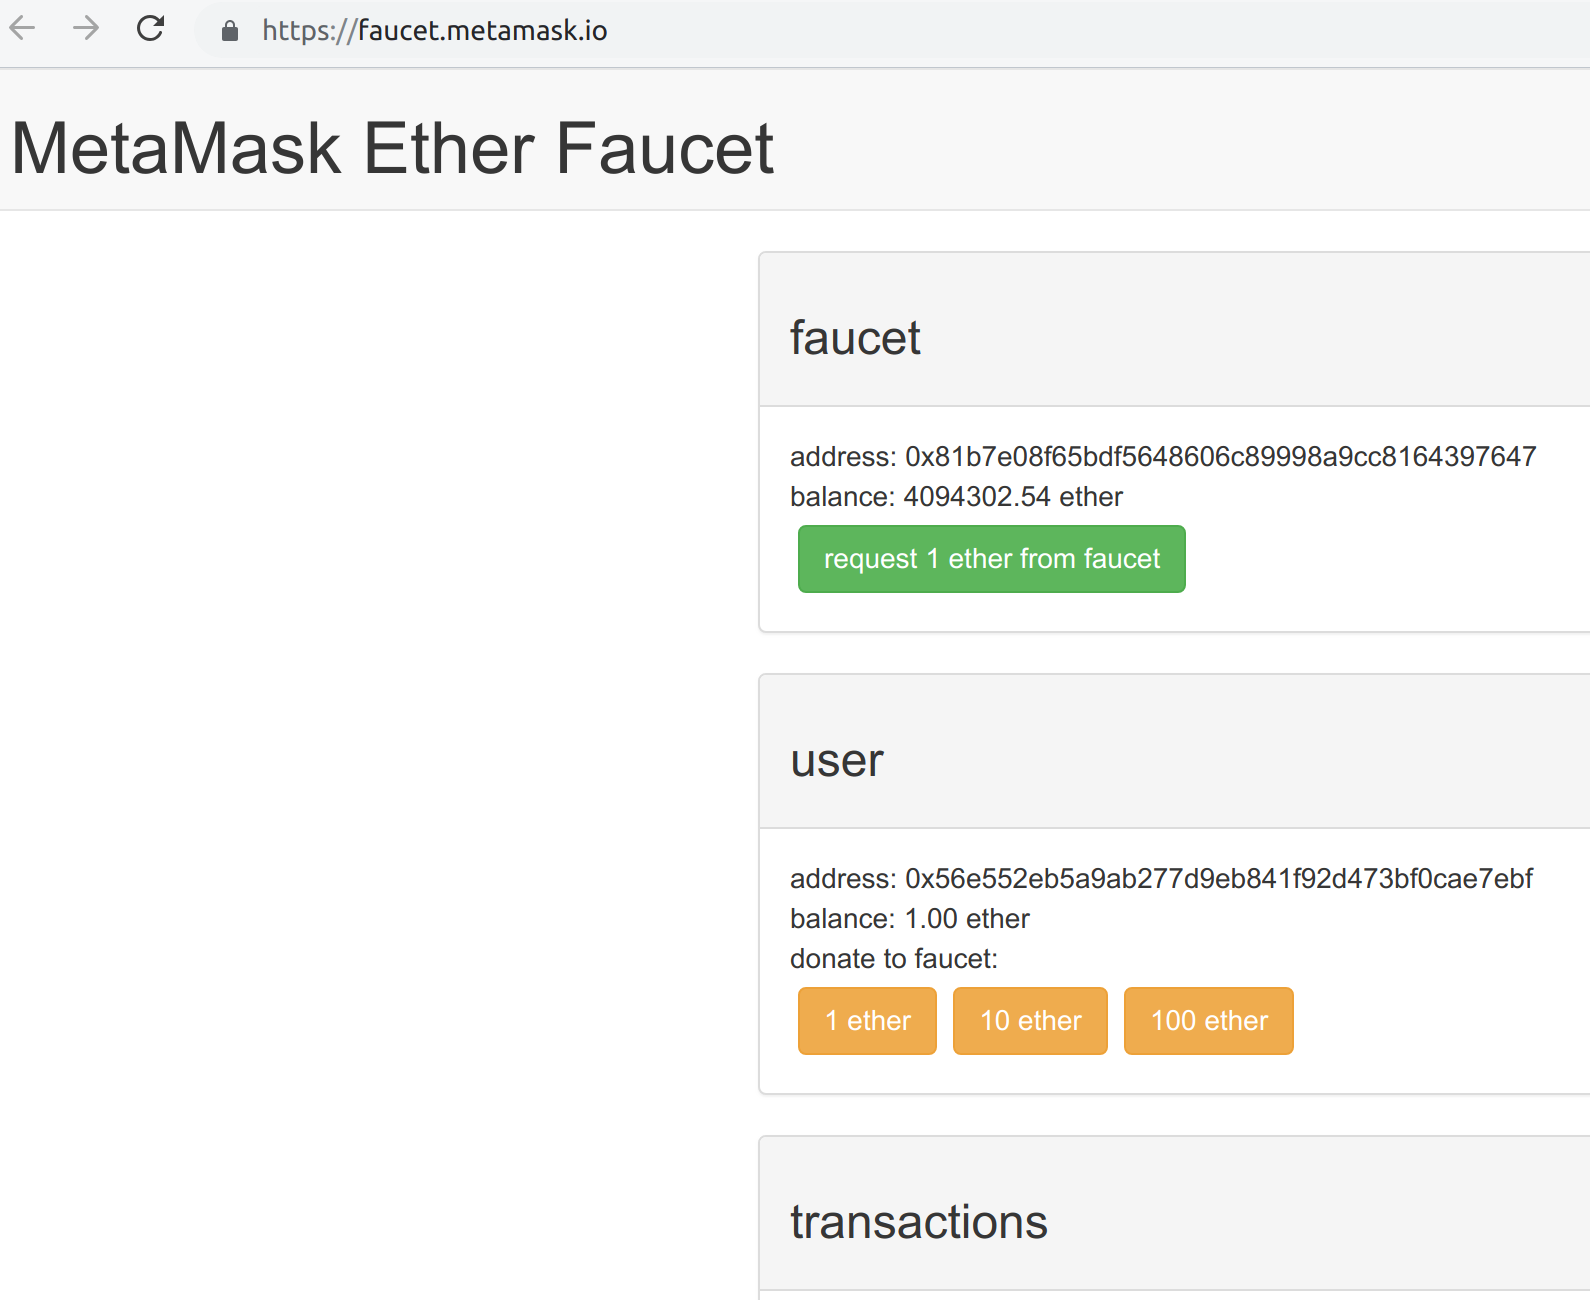
\includegraphics[width=10cm]{../pics/ethereum/faucet-ropsten}
	\end{figure}
}

\frame{
	\frametitle{Check the transaction on Metamask}
	\framesubtitle{Click on the transaction for a detailed view}
	\begin{figure}
		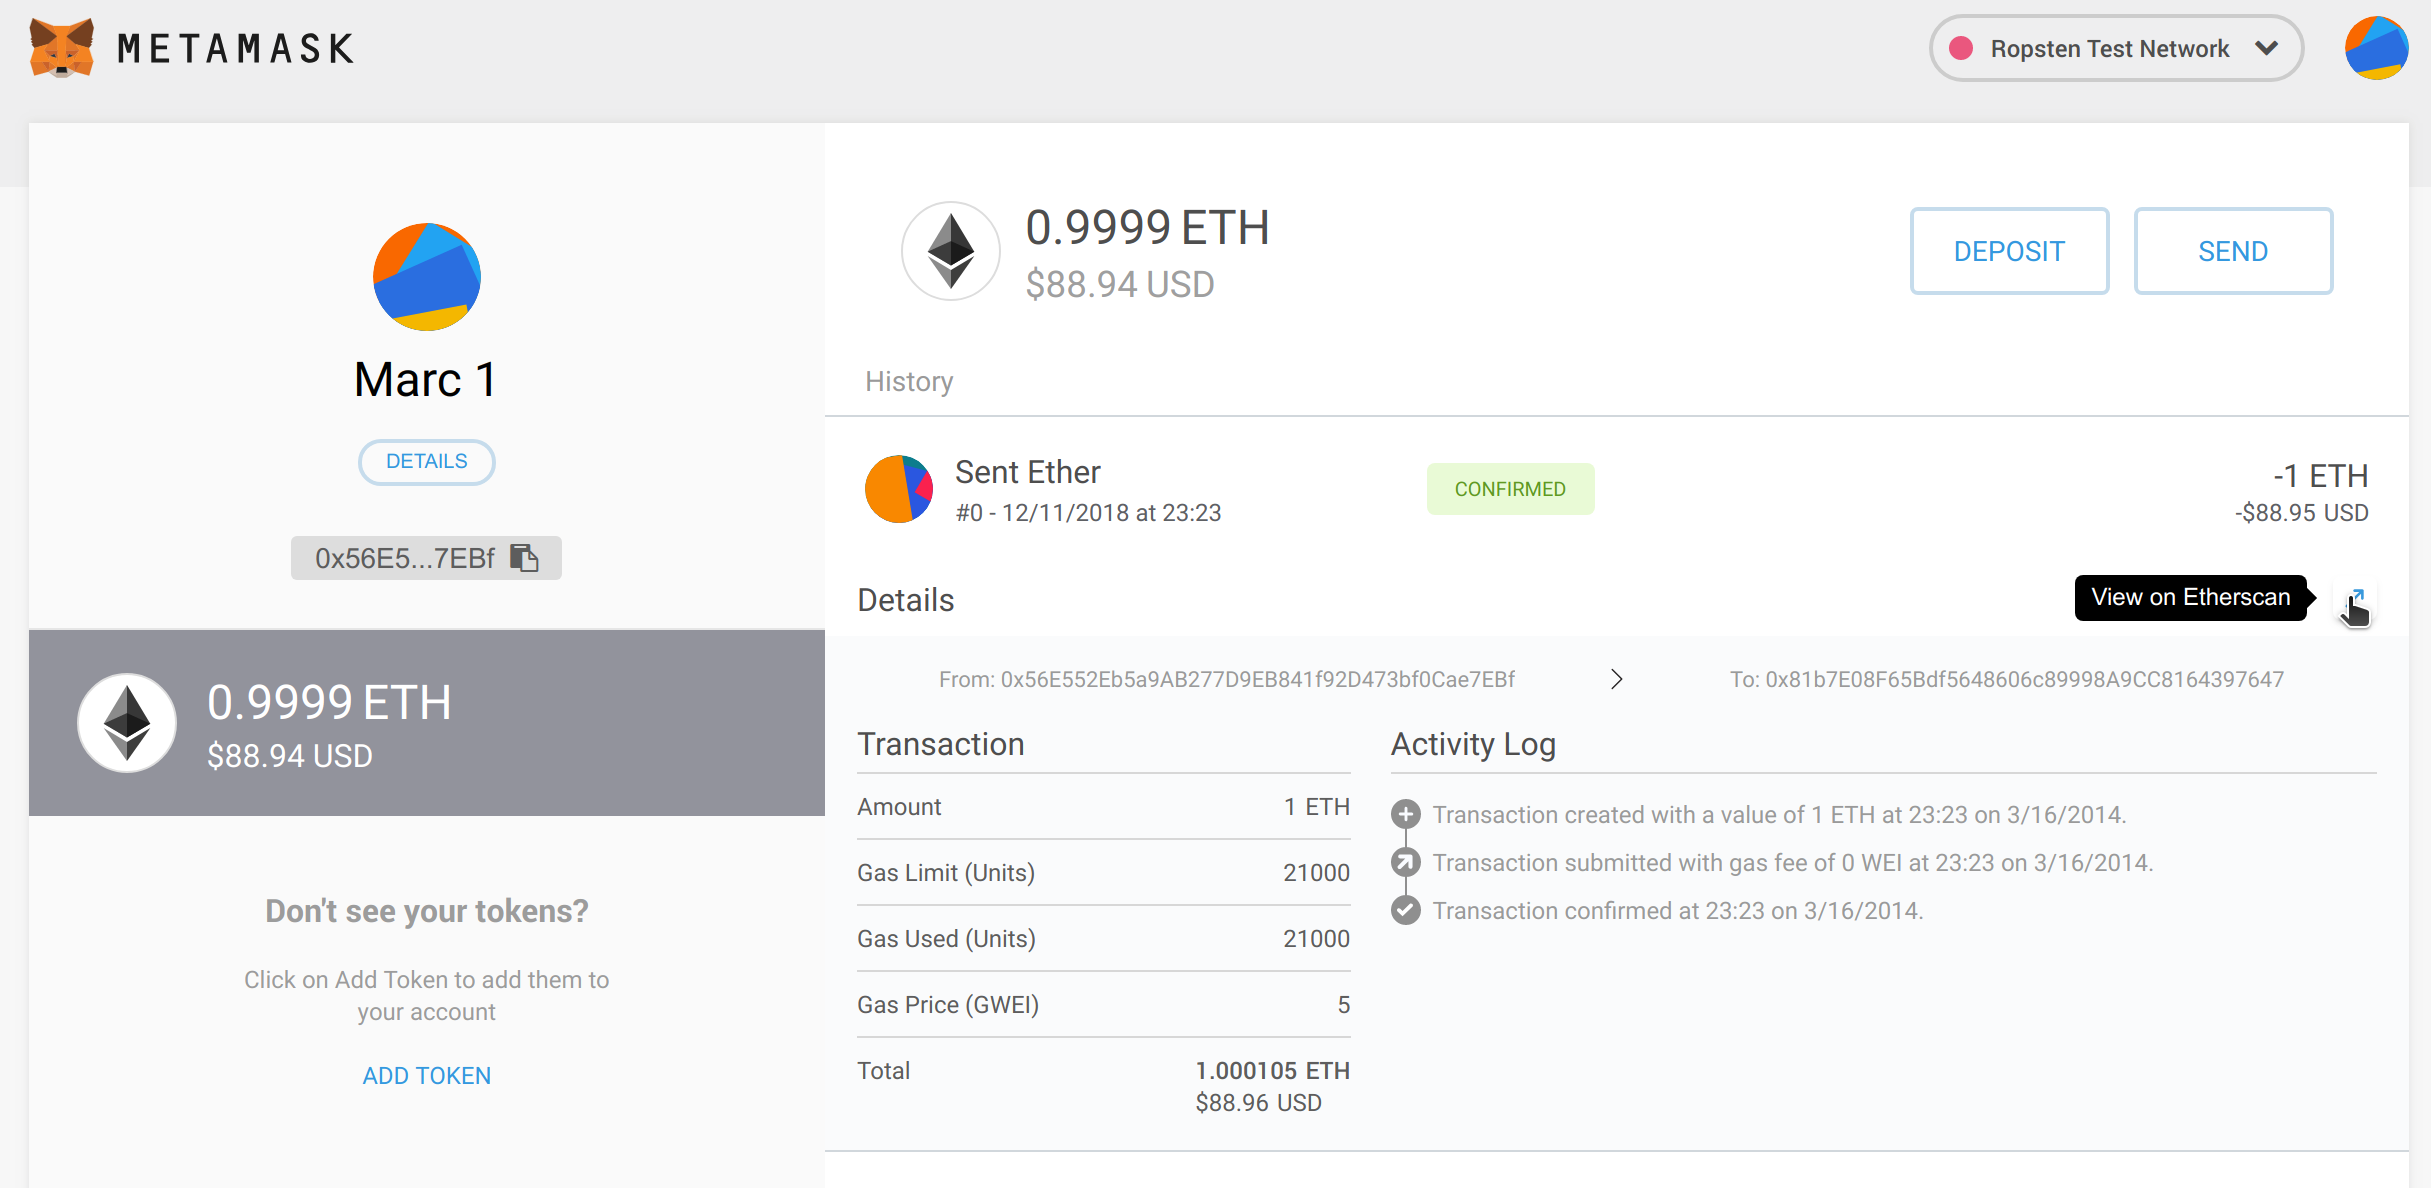
\includegraphics[width=10cm]{../pics/ethereum/metamask-tx-pane-2018}
	\end{figure}
}

\frame{
	\frametitle{Check the transaction on Etherscan}
	\begin{figure}
		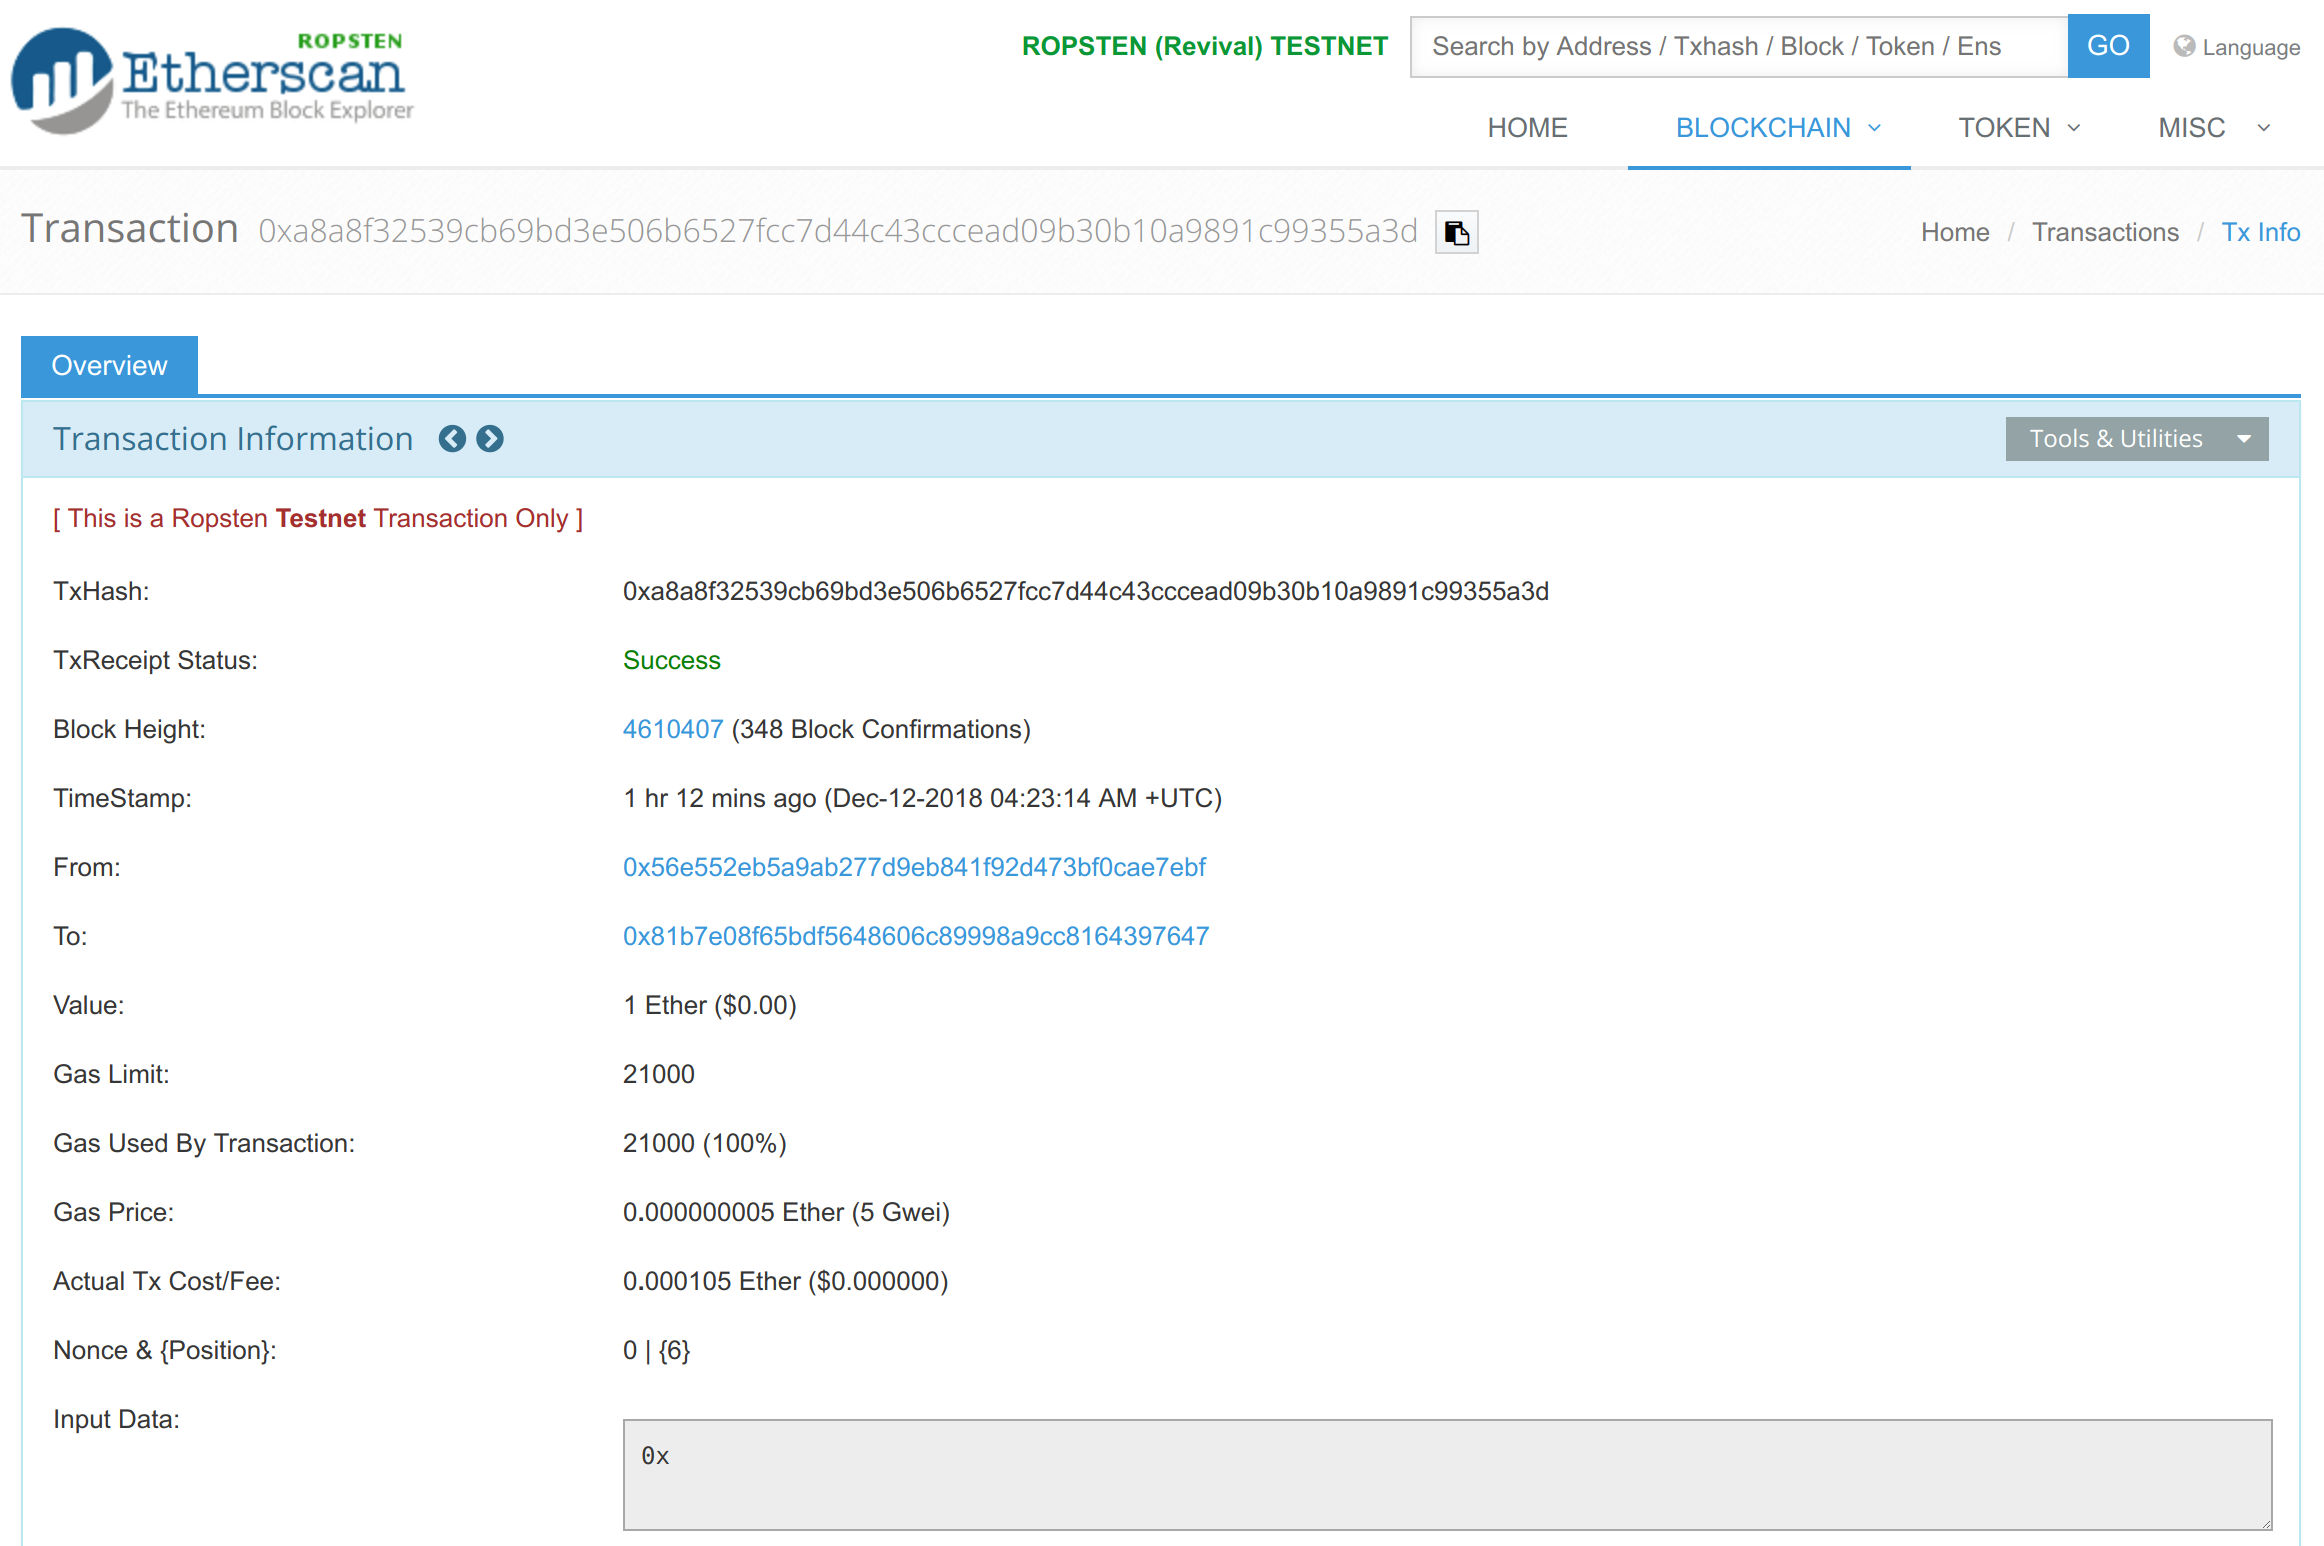
\includegraphics[width=10.9cm]{../pics/ethereum/etherscan-tx-example2}
	\end{figure}
}

\frame{
	\frametitle{A note about gas price}
	\framesubtitle{\url{https://ethgasstation.info}}
	\begin{figure}
		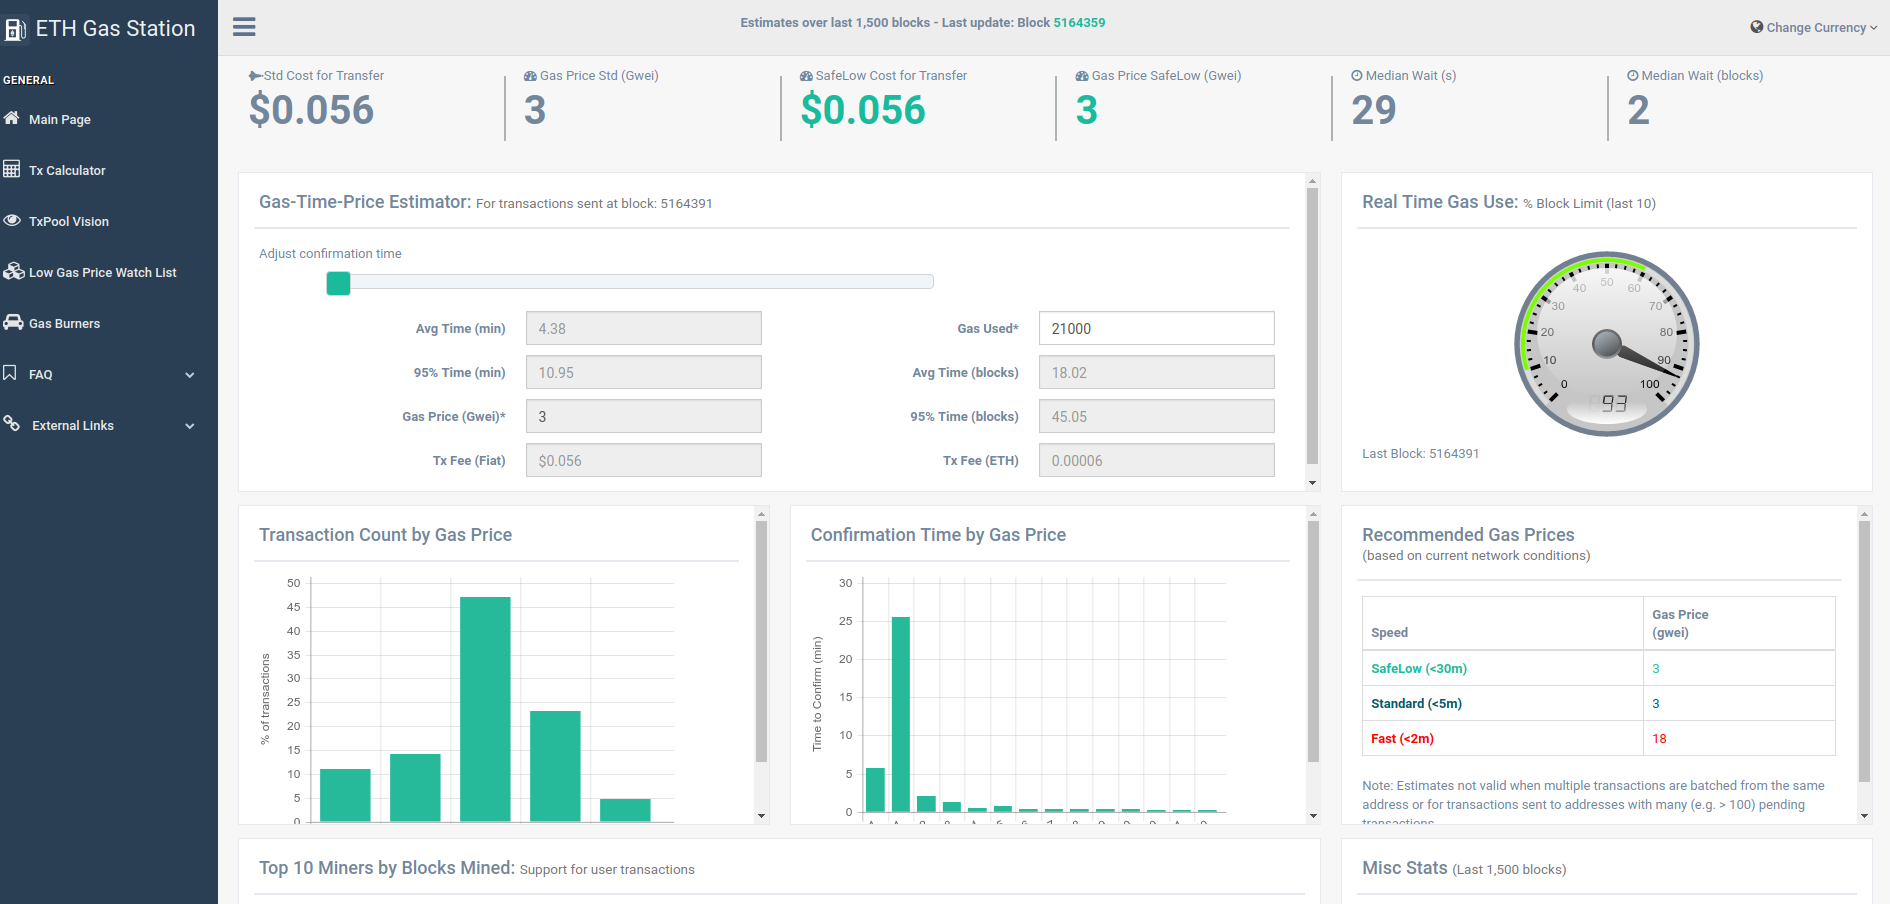
\includegraphics[width=11.5cm]{../pics/ethereum/ethgasstation}
	\end{figure}
}

\frame{
	\frametitle{Price of (real) ether: ETH}
	\framesubtitle{More information: \url{https://www.tradingview.com/symbols/ETHUSD/}}
	\begin{figure}
		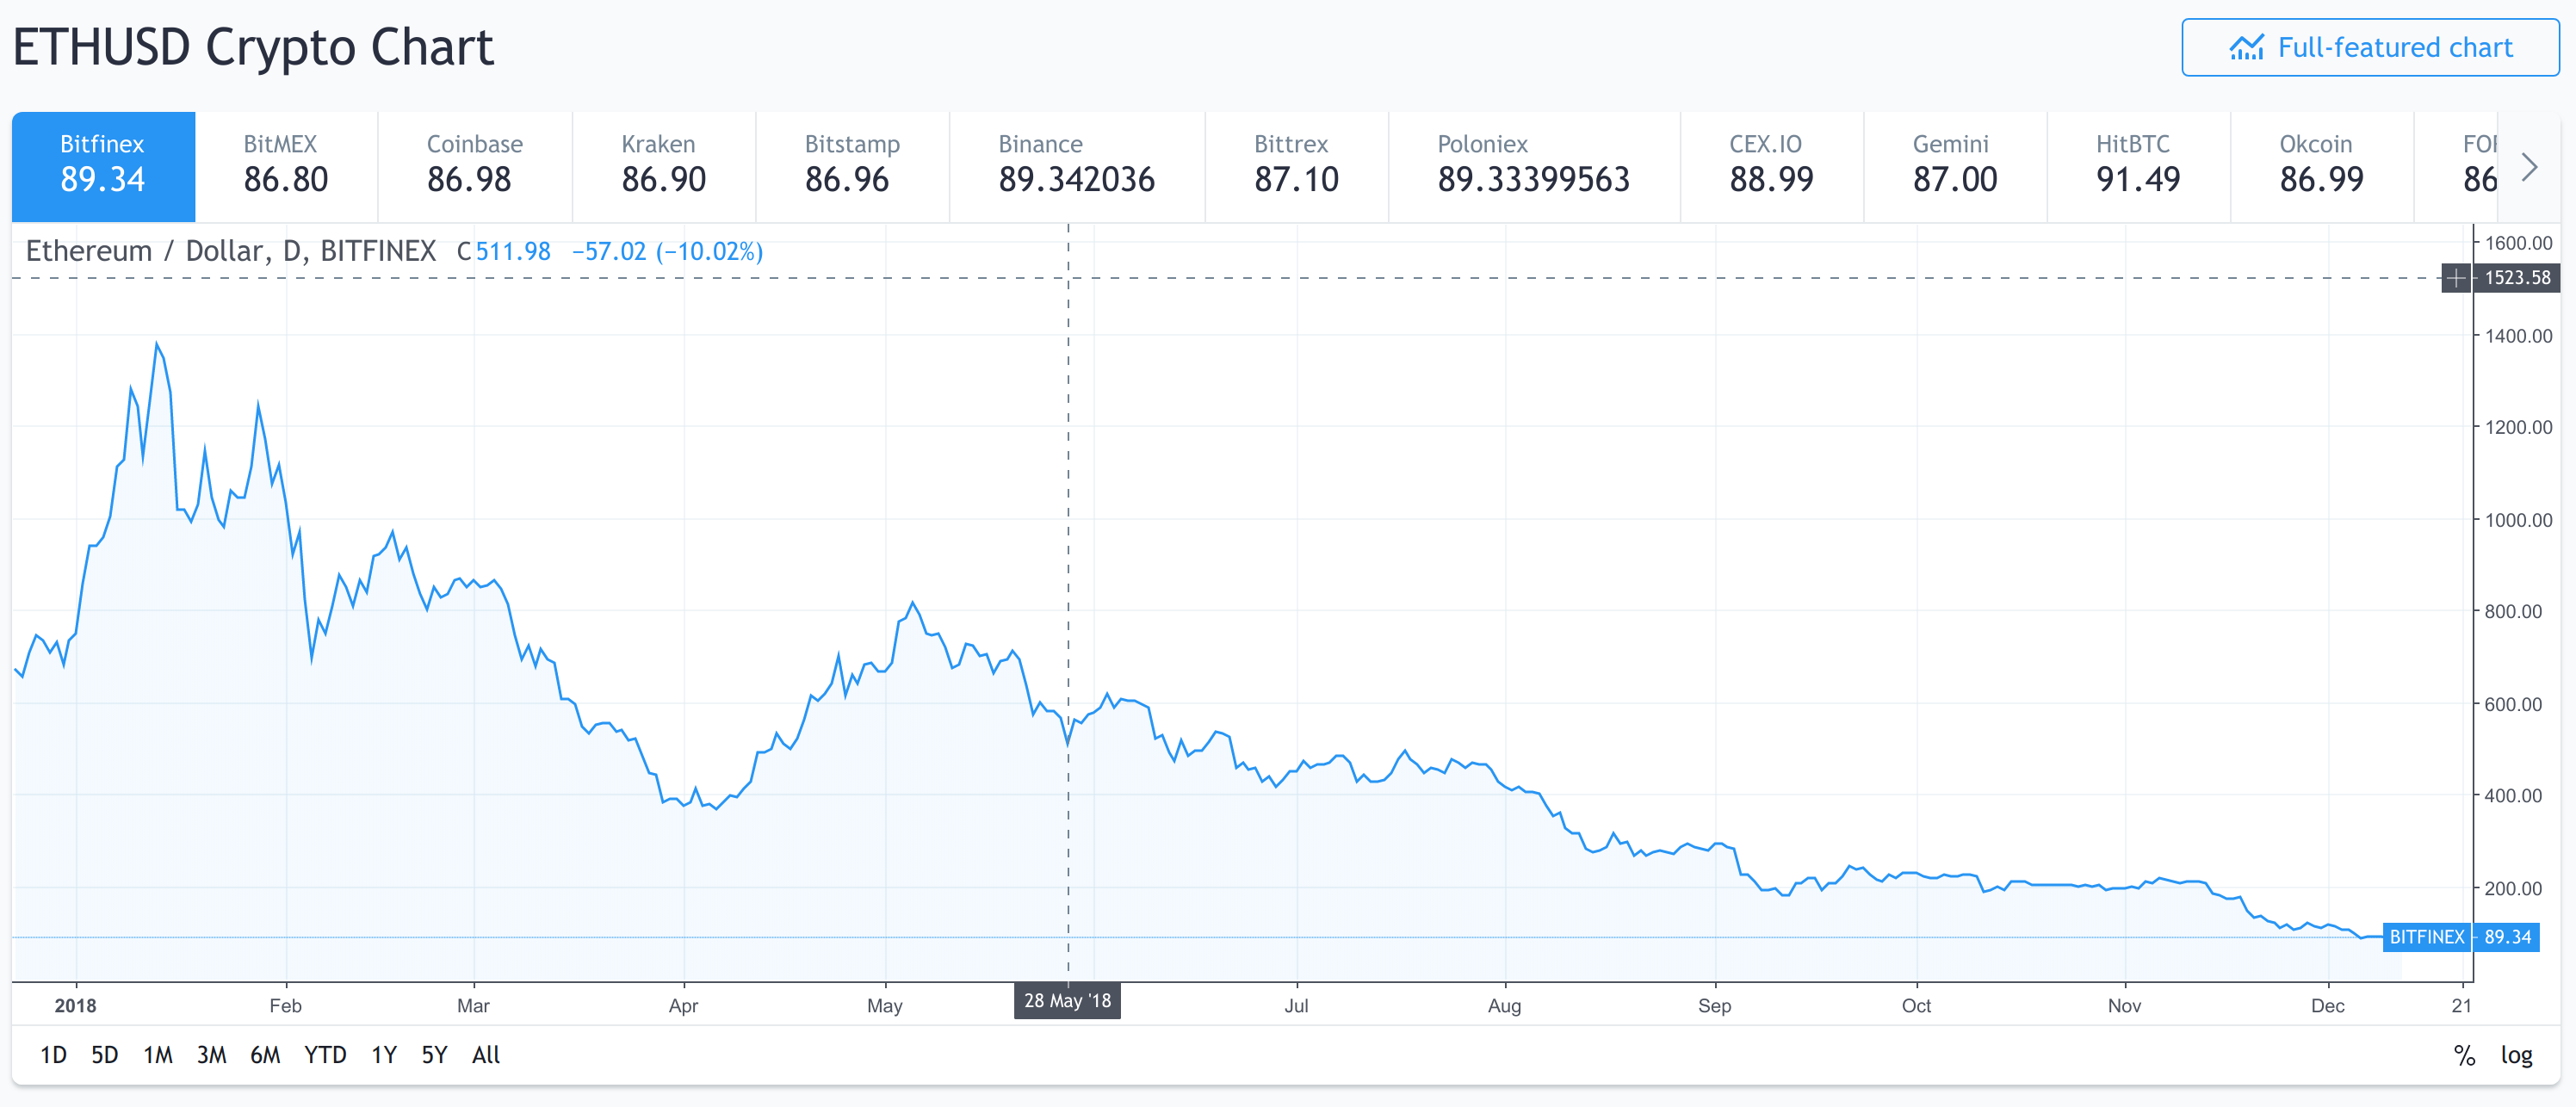
\includegraphics[width=11.5cm]{../pics/ethereum/ETH-USD-2018-12-12}
	\end{figure}
}

\frame{
	\frametitle{Wallets}
	\framesubtitle{More information: \url{https://blockgeeks.com/guides/cryptocurrency-wallet-guide/}}
	\begin{figure}
		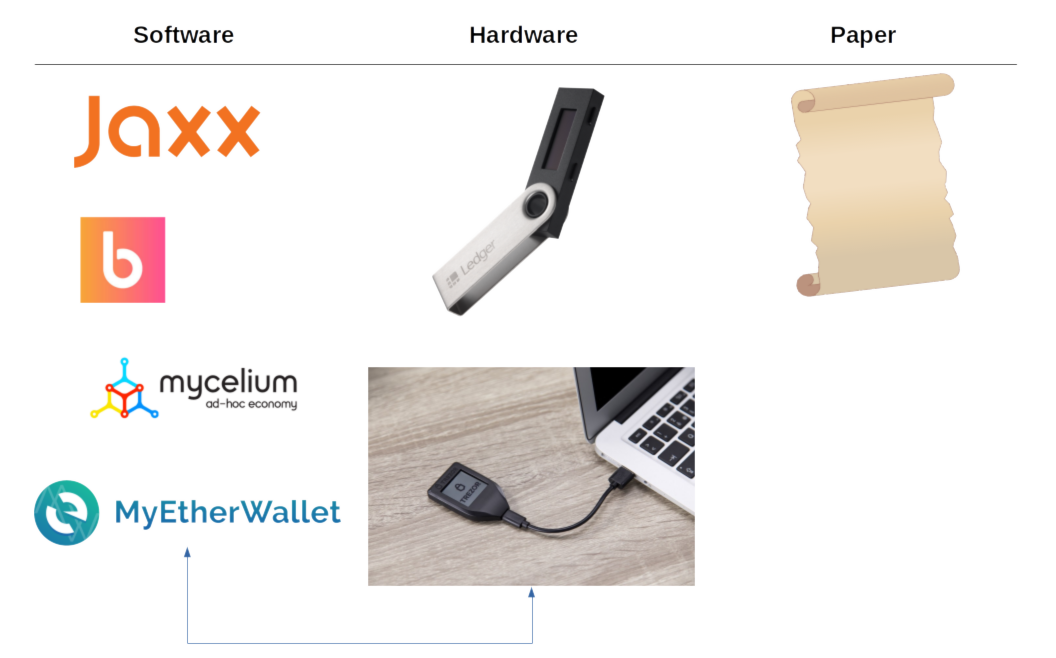
\includegraphics[width=11.5cm]{../pics/ethereum/wallets}
	\end{figure}
}

\frame{
	\frametitle{Exchanges}
	\begin{enumerate}
		\item Centralized Exchanges (Coinbase, Quadriga, ...)
		\item Decentralized Exchanges
	\end{enumerate}
}

\frame{
	\frametitle{ATMs}
	\framesubtitle{More information: \url{https://coinatmradar.com/country/138/bitcoin-atm-mexico/}}
	\begin{figure}
		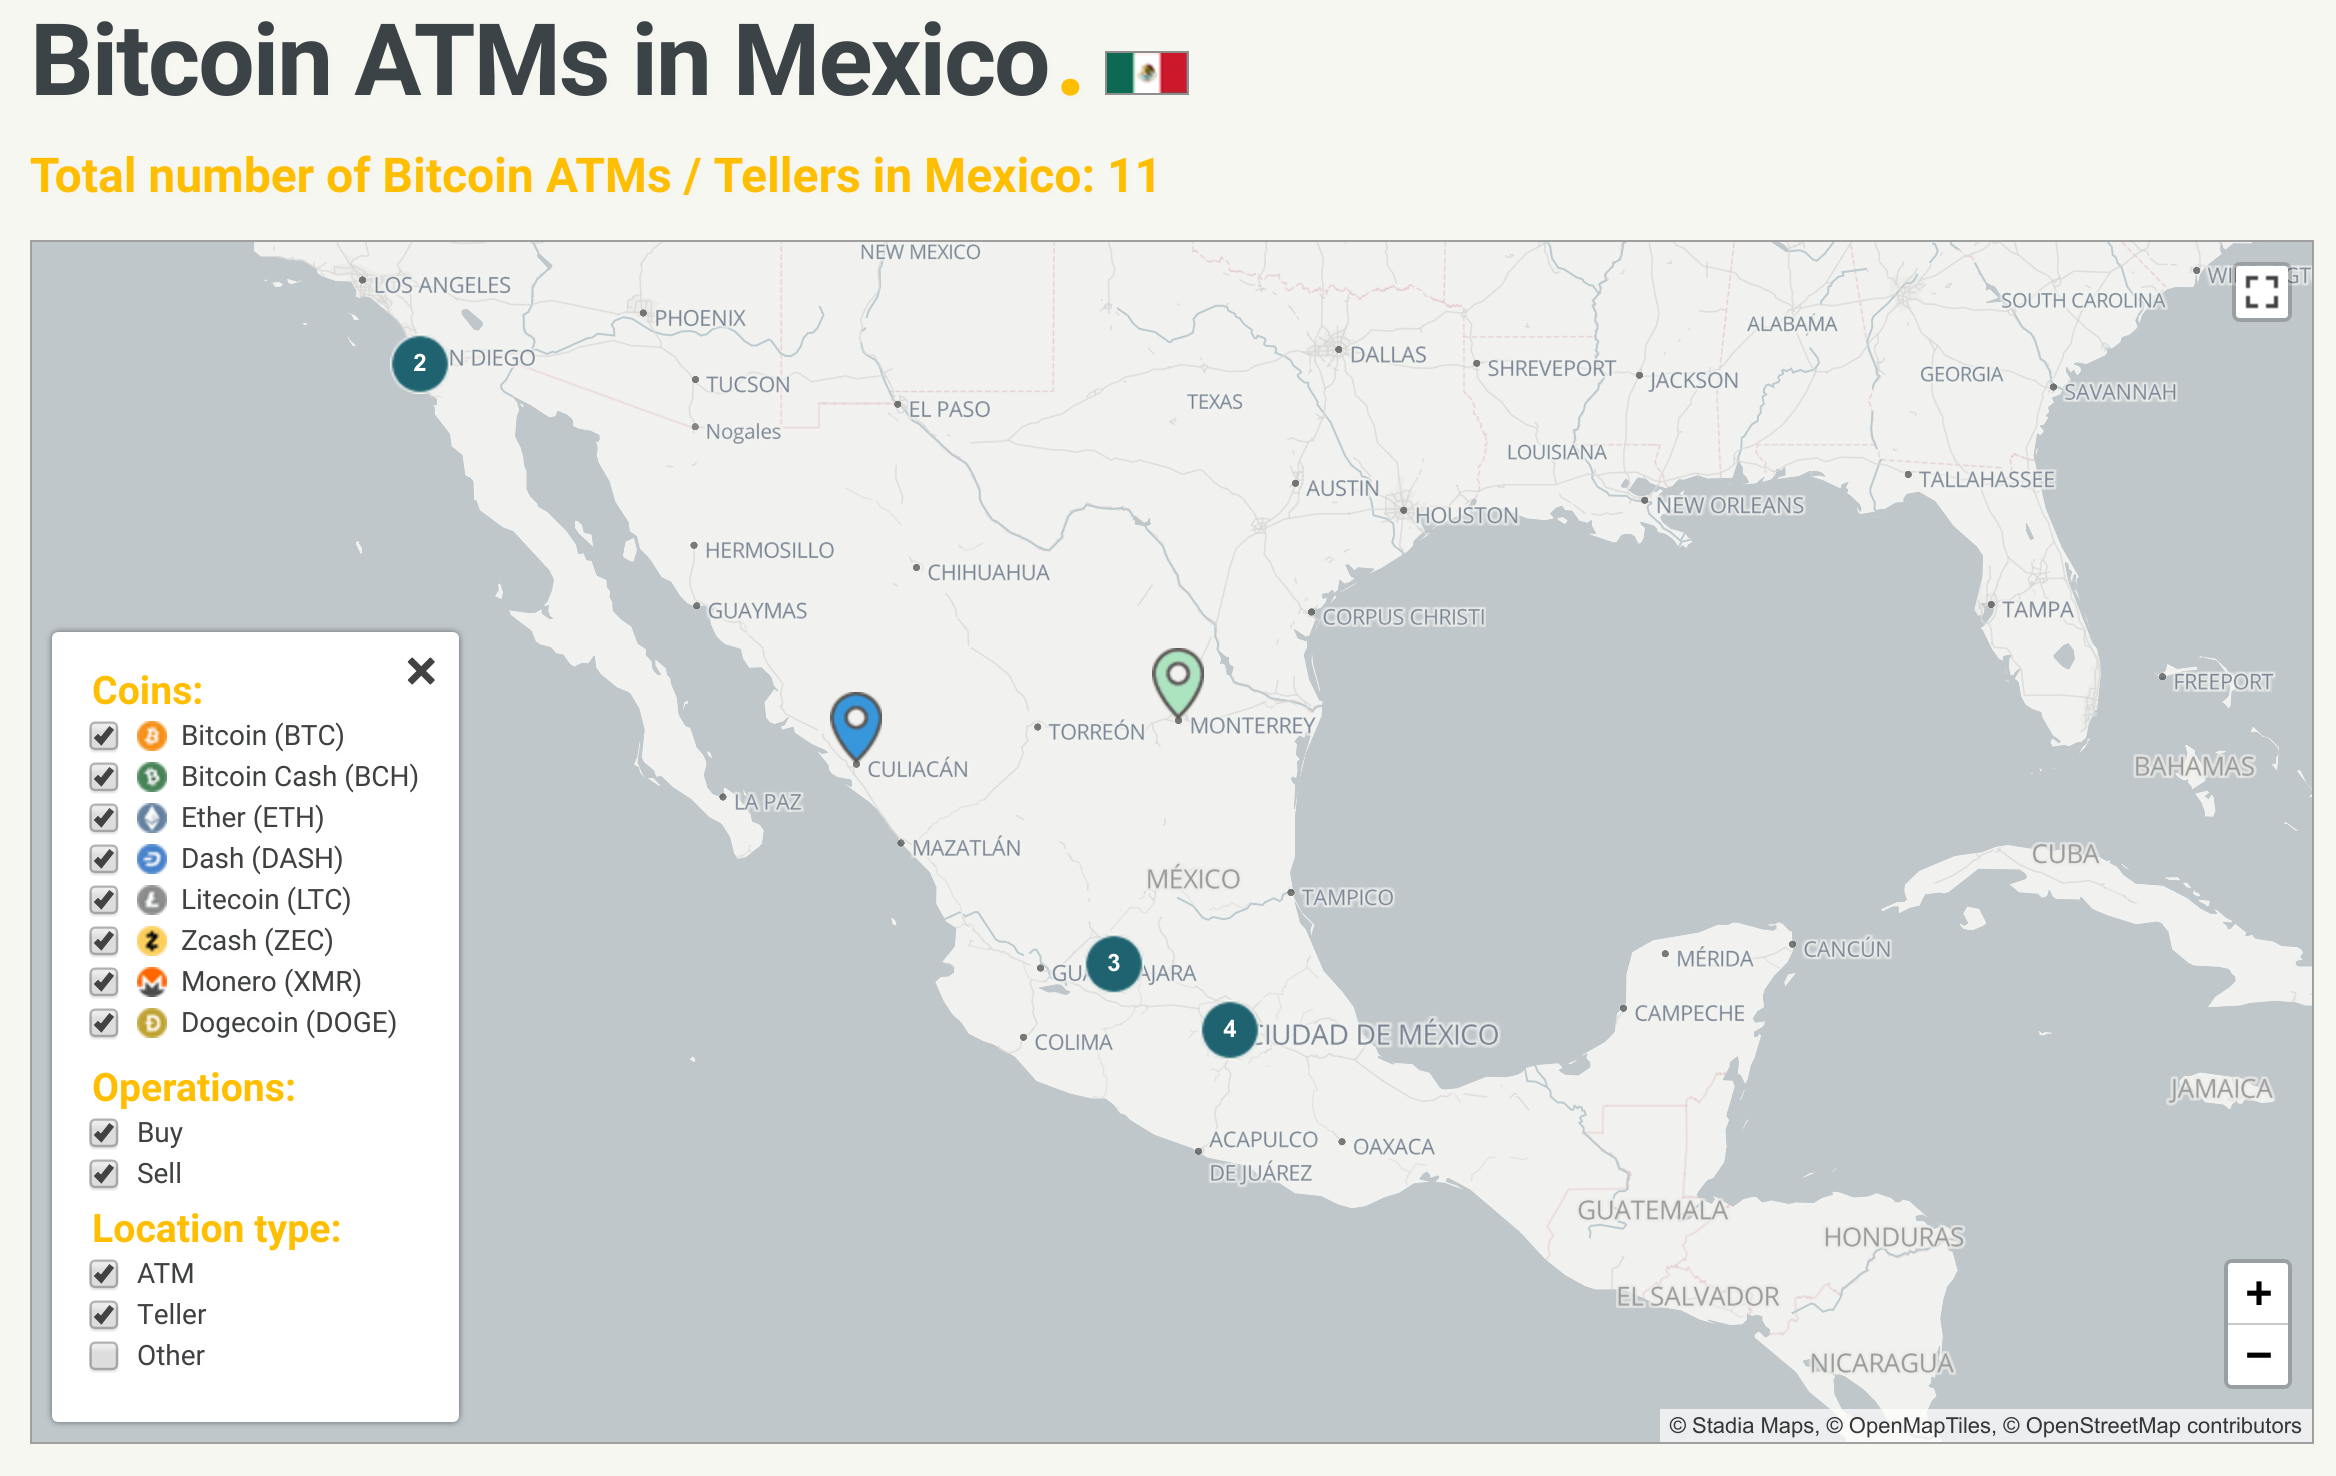
\includegraphics[width=10cm]{../pics/ethereum/bitcoin-atms-mexico}
	\end{figure}
}

\frame{
	\frametitle{Other crypto-assets}
	\framesubtitle{More information: \url{https://www.tradingview.com/markets/cryptocurrencies/prices-all/}}
	\begin{figure}
		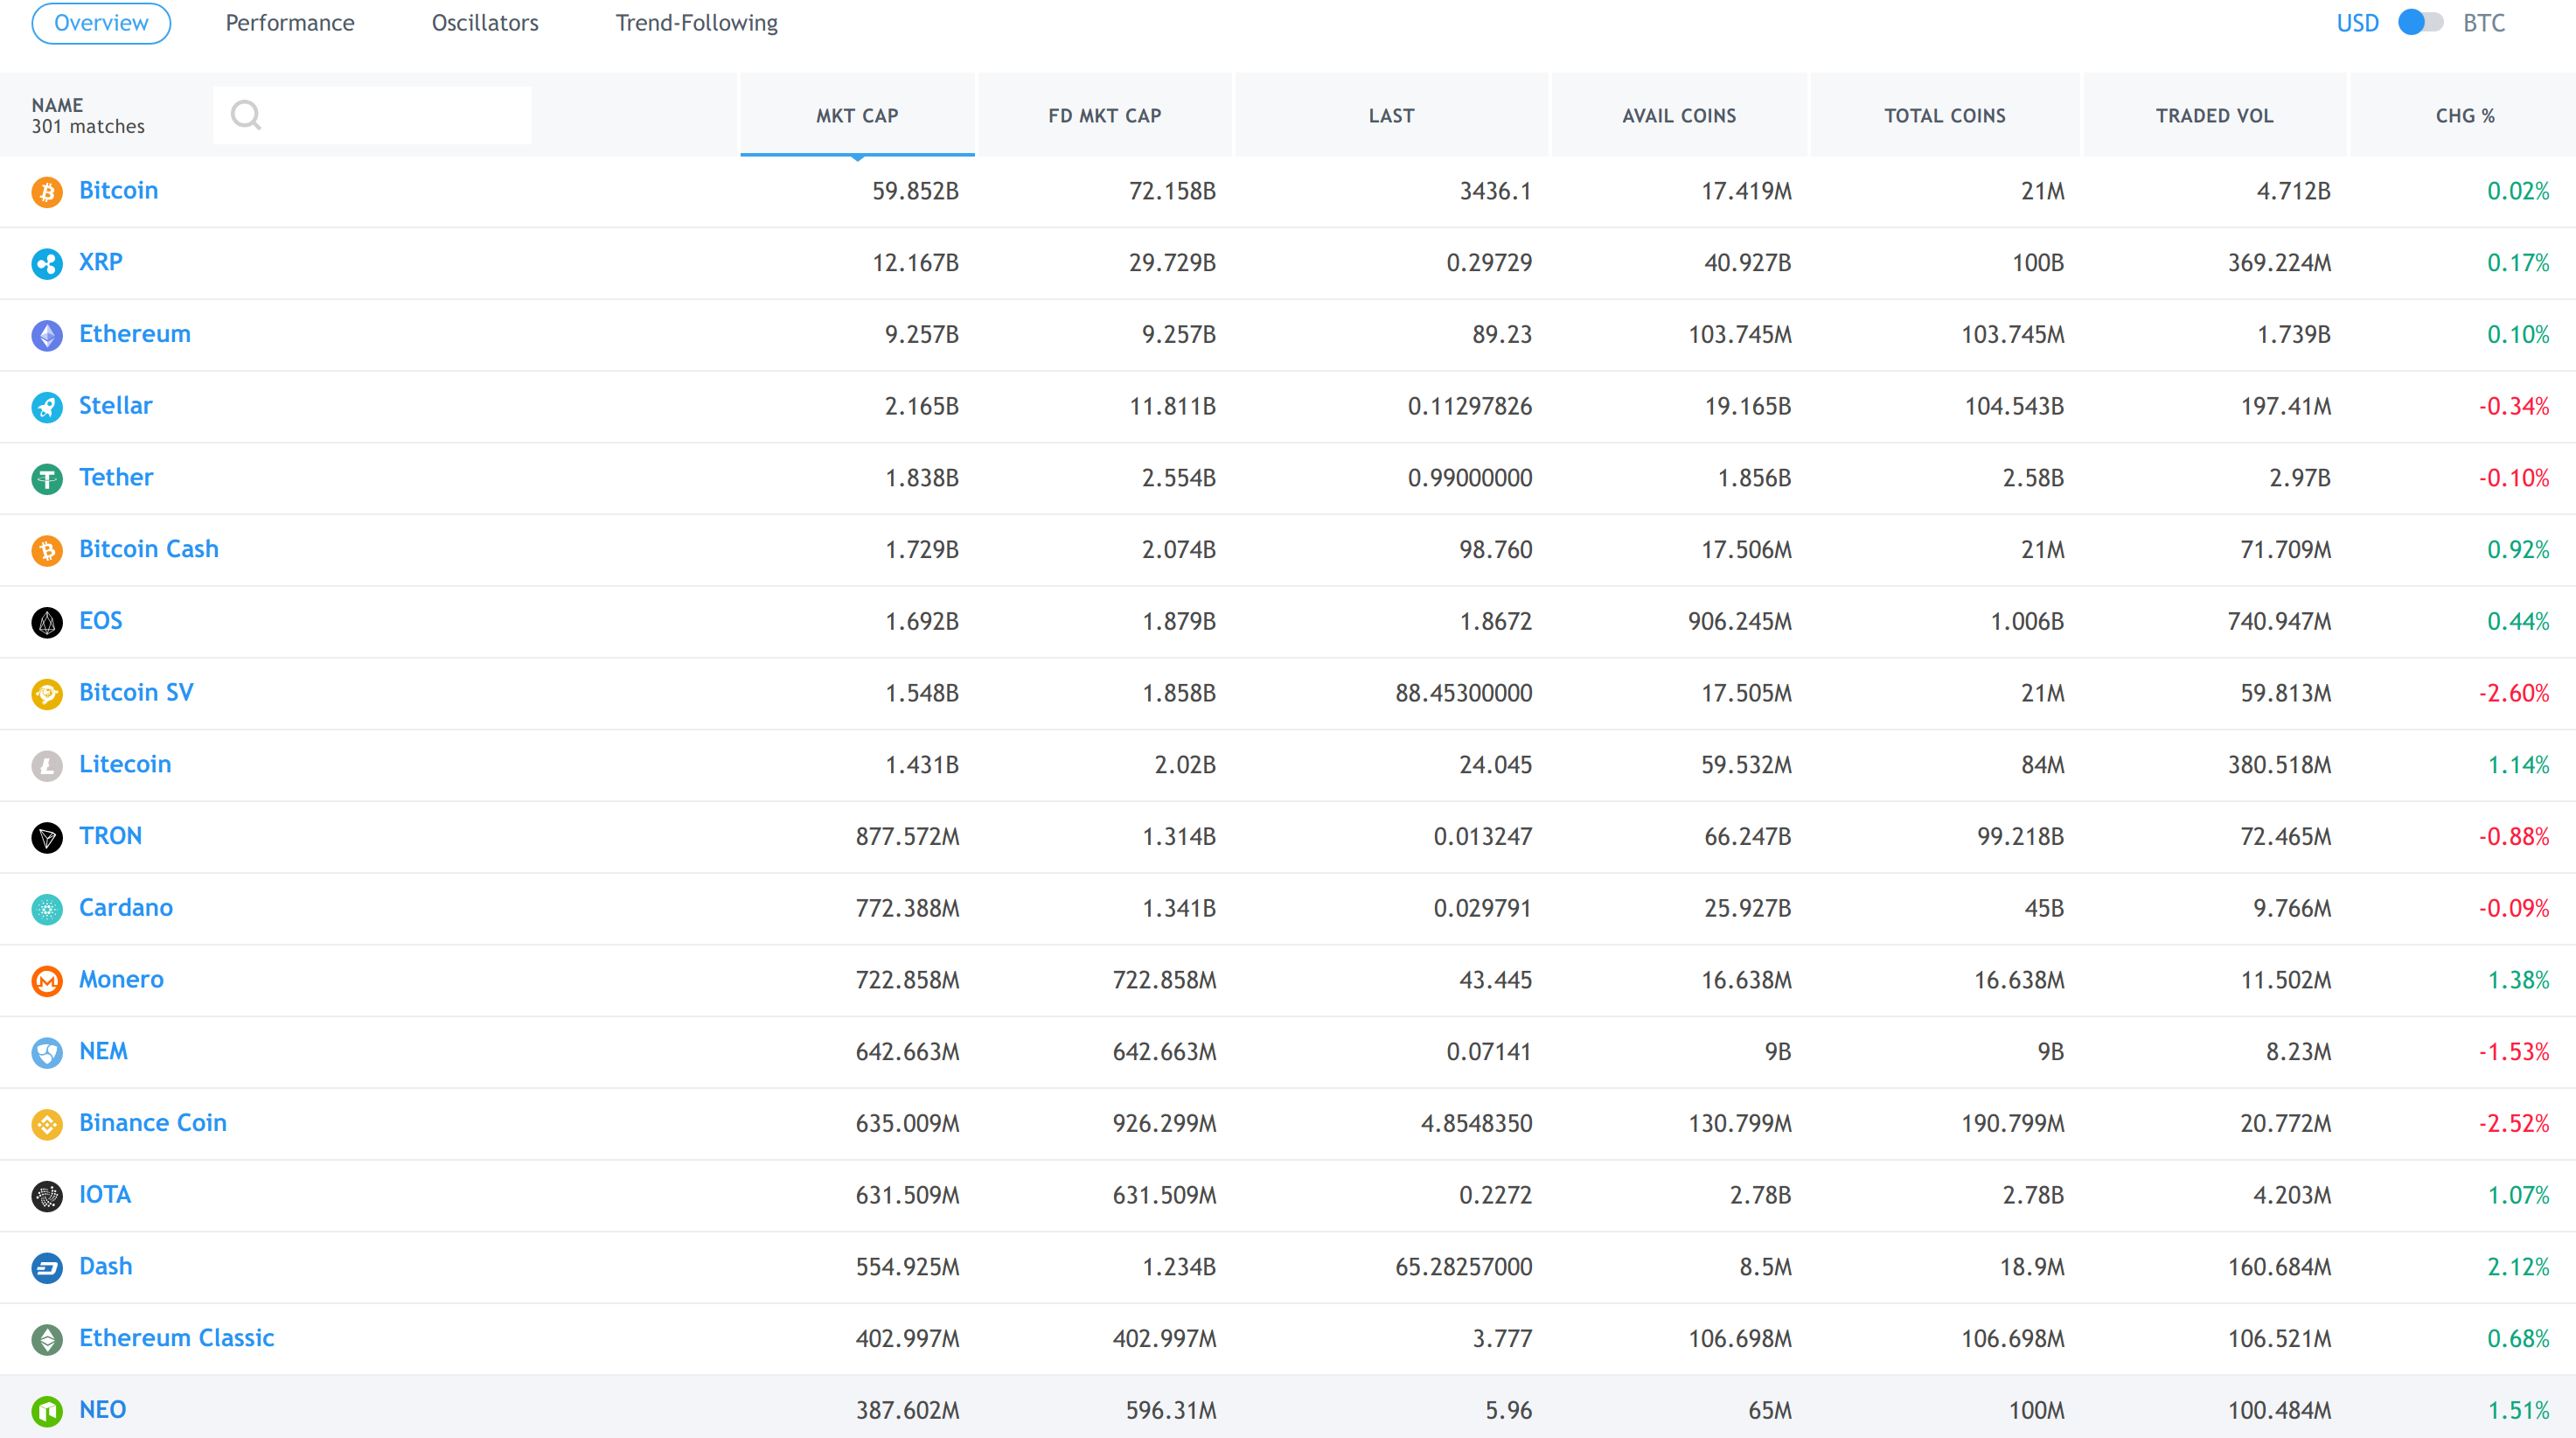
\includegraphics[width=10cm]{../pics/ethereum/coinslist-2018}
	\end{figure}
}

\frame{
	\frametitle{Ethereum, Alt-Coins, and ICOs}
	\begin{enumerate}
		\item 94\% of the top 100 tokens are built on top of Ethereum
		\item \$5.5 billion raised in 2017
		\item \$6.5 billion raised in the first quarter of 2018
		\item Ethereum has the largest developer community
		\item Close to 2,000 dapps (decentralized applications) counted on Ethereum
	\end{enumerate}
}

\frame{
	\frametitle{Crypto as seen by the Regulator (and the taxman)}
	\begin{enumerate}
		\item Cryptocurrency
		\item Utility Token
		\item Security Token
	\end{enumerate}
}

\frame{
	\frametitle{Create your own (ERC-20) token}
	\begin{figure}
		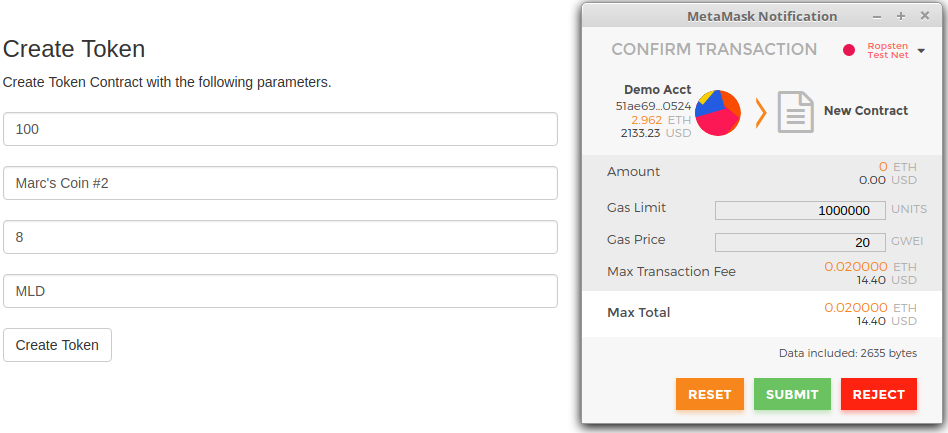
\includegraphics[width=10cm]{../pics/ethereum/token-factory-create}
	\end{figure}
	\vspace{-1em}
	\begin{enumerate}
		\item Use the Token Factory Dapp at \url{https://tokenfactory.surge.sh/\#/factory}
		\item MetaMask will pop up (see picture above)
		\item Submit the transaction (on the Ropsten Testnet)
		\item Check your transaction on \url{https://ropsten.etherscan.io} 
	\end{enumerate}
}

\frame{
	\frametitle{Check your Smart Contract}
	\begin{figure}
		
\includegraphics[width=10cm]{../pics/ethereum/metamask-contract-published}
	\end{figure}
	\vspace{-1em}
	\begin{enumerate}
		\item Select the ``Sent'' tab
		\item Check the orange Copy icon (Tx Hash) 
		\item Click on ``Contract Published''
		\item That should bring you to Etherscan (see next page)
	\end{enumerate}
}

\frame{
	\frametitle{Verify the status of your transaction on Etherscan}
	\begin{figure}
		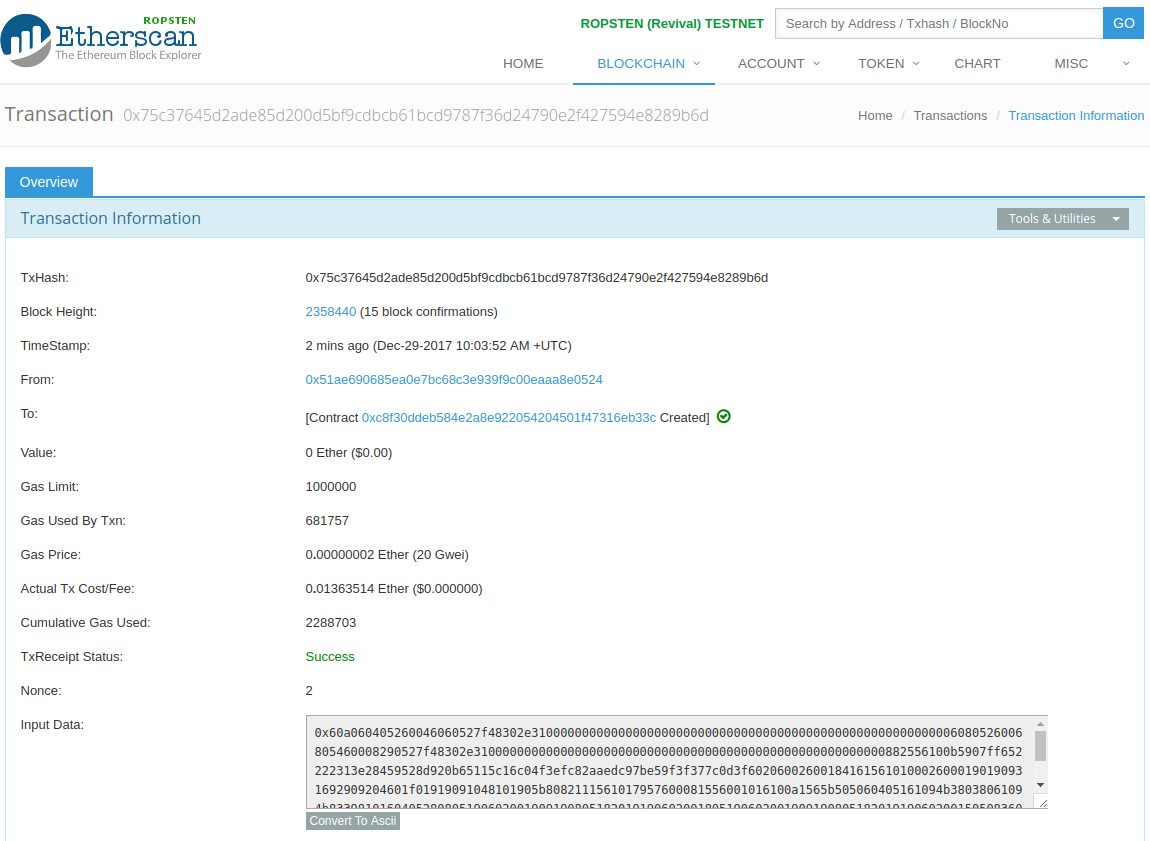
\includegraphics[width=10cm]{../pics/ethereum/etherscan-contract}
		\captionsetup{justification=centering}
		\caption*{Transaction Information: note the ``To'' line with your contract address}
	\end{figure}
}

\frame{
	\frametitle{Watch your Token}
	\begin{columns}
	\column{0.5\textwidth}
		\begin{figure}
			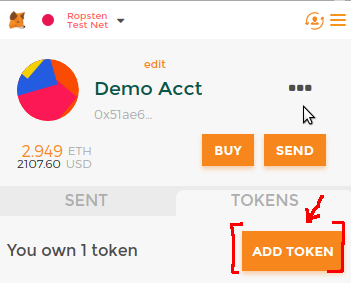
\includegraphics[width=3cm]{../pics/ethereum/metamask-add-token-1}
		\end{figure}
	\column{0.5\textwidth}
		\begin{figure}
			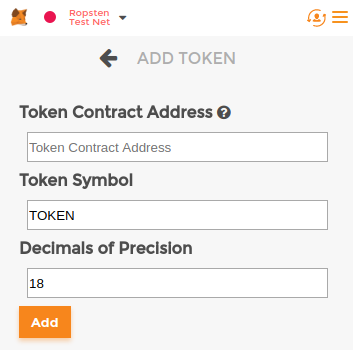
\includegraphics[width=3cm]{../pics/ethereum/metamask-add-token-2}
		\end{figure}
	\end{columns}
	\begin{enumerate}
		\item Click on the ``Add Token'' button
		\item Wait for the next window (picture on the right)
		\item Copy your contract address (from Etherscan)
		\item Go back to your Token Factory tab, which should show an UI to interact with your contract or go to the URL: https://tokenfactory.surge.sh/\#/token/0x... (replace 0x... by your contract address)
		\item Move coins around
		\item In MetaMask, click on your token to check the tx on Etherscan 
	\end{enumerate}
}


% ======================================================================================================
%                                     Hands-on Introduction to Smart Contracts 
% ======================================================================================================
\section{Introduction to Smart Contracts}
\frame{
	\frametitle{Remember: Ethereum}
	%\framesubtitle{}
	\begin{columns}
	\column{0.5\textwidth}
		Ethereum is a \textbf{decentralized platform that runs smart contracts}: applications that run exactly as programmed without any possibility of downtime, censorship, fraud or third party interference.\\
		--- \url{https://ethereum.org}
	\column{0.5\textwidth}
		\begin{figure}
			
\includegraphics[height=6cm]{../pics/ethereum/471px-Ethereum_logo_2014}
		\end{figure}
	\end{columns}
}

\frame{
	\frametitle{Coding your first ERC-20 Smart Contract}
	\begin{figure}
		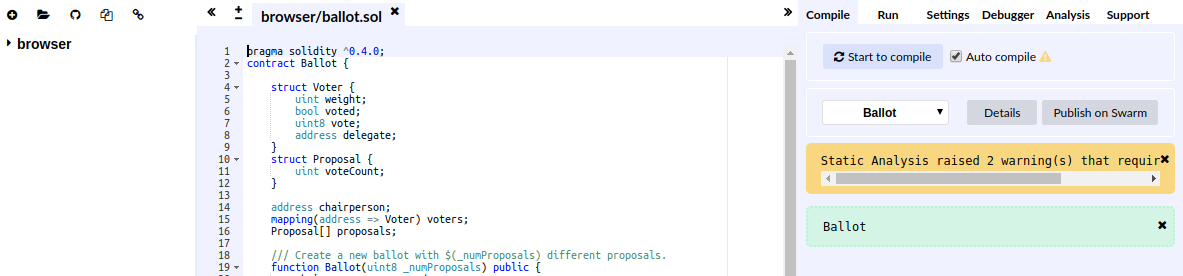
\includegraphics[width=10cm]{../pics/ethereum/remix-home}
	\end{figure}
	\begin{enumerate}
		\item Open the Remix IDE at \url{https://remix.ethereum.org}
		\item Close the ballot file 
		\item Create a new file named TokenRecipient.sol 
		\item Copy the code from \url{https://ethereum.org/token} (second white box, under ``The Code'', starting with ``pragma'')
		\item Switch to the ``Run'' tab (top-right bar, after Compile)
	\end{enumerate}
	Reference:\\
	\href{https://github.com/ethereum/EIPs/blob/master/EIPS/eip-20-token-standard.md}{ERC-20 Token Standard}
}

\frame{
	\frametitle{Compiling Successfully}
	\begin{figure}
		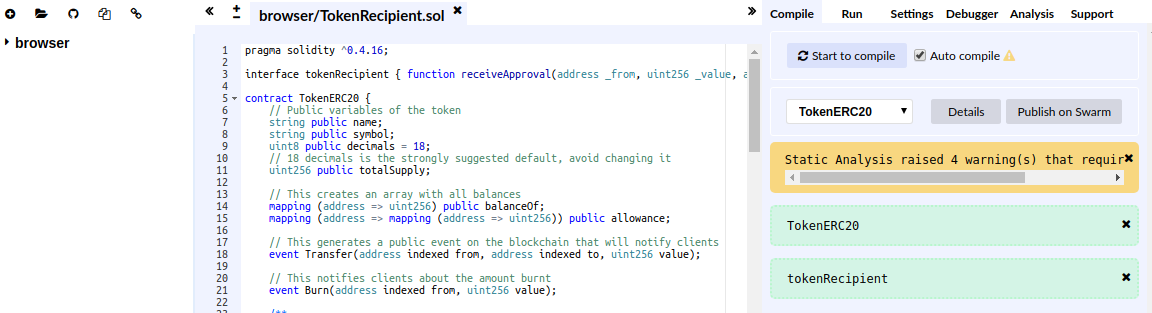
\includegraphics[width=10cm]{../pics/ethereum/remix-compiling-ERC20}
	\end{figure}
	\begin{enumerate}
		\item Two green boxes should show on the right 
		\item TokenERC20 is the name of the contract (class)
		\item tokenRecipient is the name of the interface
		\item Switch to the ``Run'' tab (top right)
	\end{enumerate}
}

\frame{
	\frametitle{Submitting the Smart Contract}
	\begin{figure}
		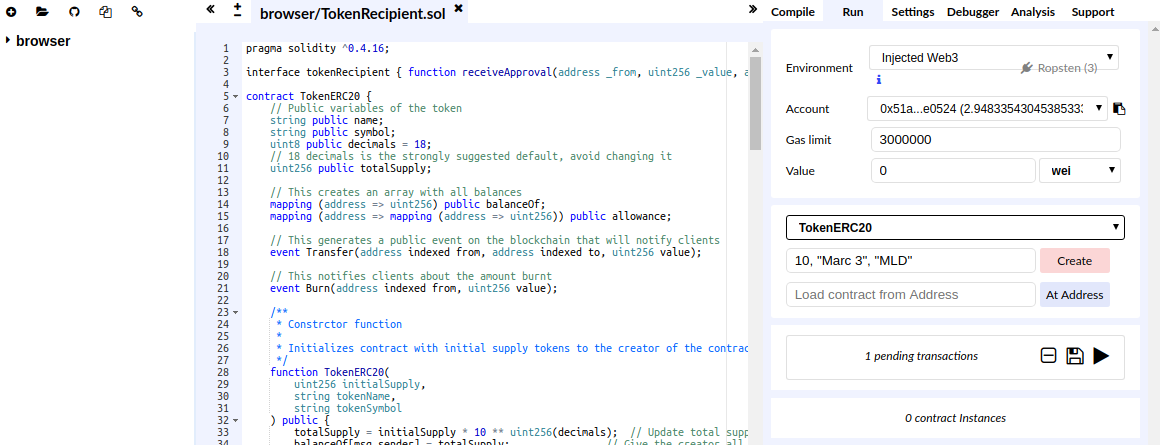
\includegraphics[width=10cm]{../pics/ethereum/remix-creating-ERC20}
	\end{figure}
	\begin{enumerate}
		\item Under the dropdown showing ``TokenERC20'', add a number (total amount of tokens to issue) and two strings (the latter is the token symbol)
		\item Add enough gas (top right, try 30)
		\item Click Create and check whether MetaMask needs confirmation
	\end{enumerate}
}
\frame{
	\frametitle{Interacting with the contract}
	\begin{columns}
	\column{0.4\textwidth}
		\begin{enumerate}
			\item A new interface will pop up on the bottom right corner of the IDE
		\end{enumerate}
	\column{0.6\textwidth}
		\begin{figure}
			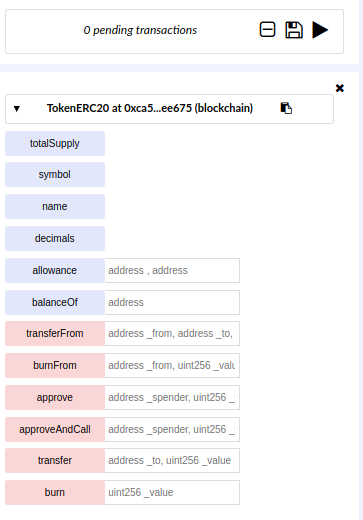
\includegraphics[height=7cm]{../pics/ethereum/remix-ERC20-interact}
		\end{figure}
	\end{columns}
}

\frame{
	\frametitle{}
	\centering\Huge
	Tools for Developers
}

\frame{
	\frametitle{Truffle Framework}
	\framesubtitle{\url{http://truffleframework.com}}
	\begin{figure}
		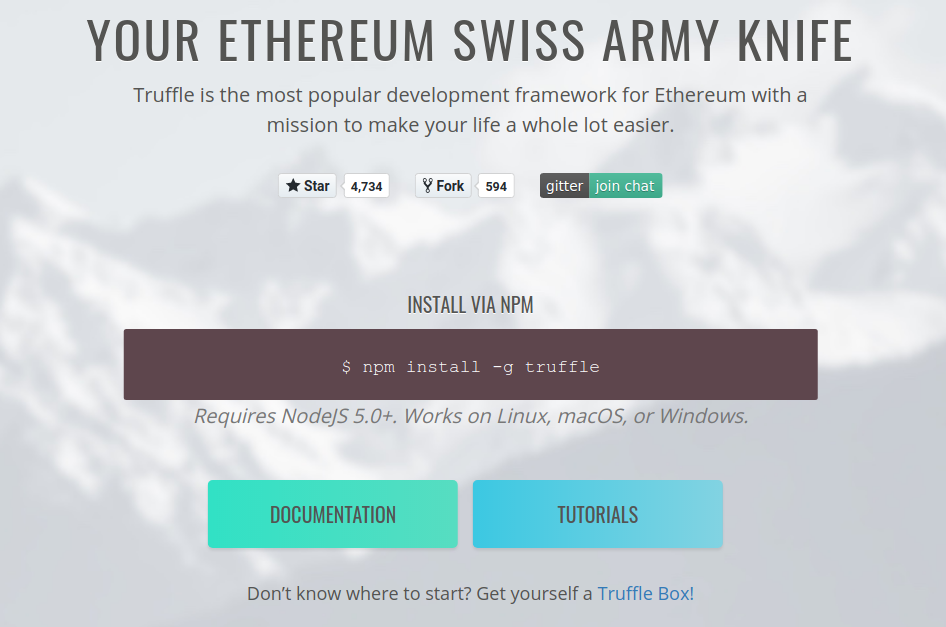
\includegraphics[width=11cm]{../pics/ConsenSys/truffle}
	\end{figure}
}

\frame{
	\frametitle{Infura}
	\framesubtitle{\url{http://infura.io}}
	\begin{figure}
		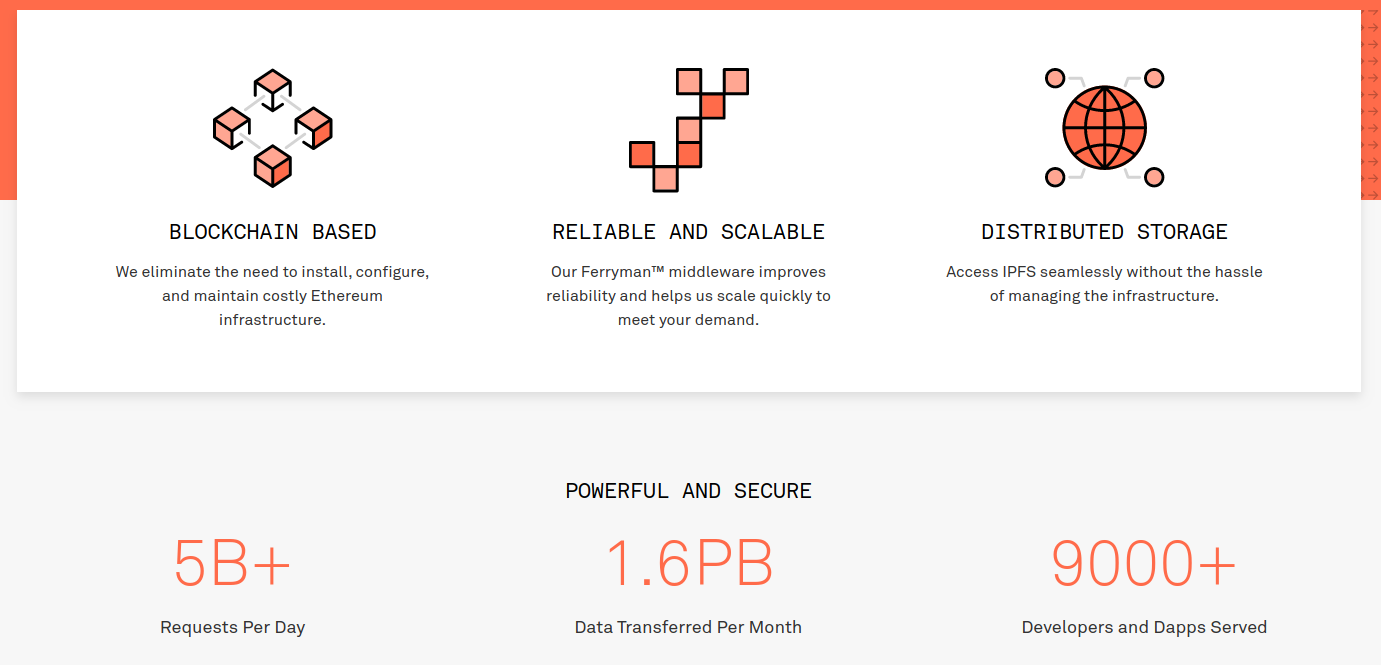
\includegraphics[width=11cm]{../pics/ConsenSys/infura}
	\end{figure}
}

\begin{frame}[fragile]
	\frametitle{Mythril}
	\framesubtitle{\url{https://github.com/ConsenSys/mythril}}
	Mythril is a security analysis tool for smart contracts.\\
	It comes as a Python package that requires a solidity compiler and a C++ compiler.
	\vspace{1em}
	\begin{Verbatim}[fontsize=\tiny]
$ sudo apt install libssl-dev
$ sudo apt install gcc g++
$ sudo add-apt-repository ppa:ethereum/ethereum
$ sudo apt install solc
$ sudo pip3 install mythril 
$ myth -x contracts/higherbidder.sol 
	\end{Verbatim}
	\vspace{3em}
	{\footnotesize See also \url{https://hackernoon.com/introducing-mythril-a-framework-for-bug-hunting-on-the-ethereum-blockchain-9dc5588f82f6}}
\end{frame}

\frame{
	\frametitle{Big Data and Analytics on Ethereum}
	\framesubtitle{\url{https://aleth.io}}
	\begin{figure}
		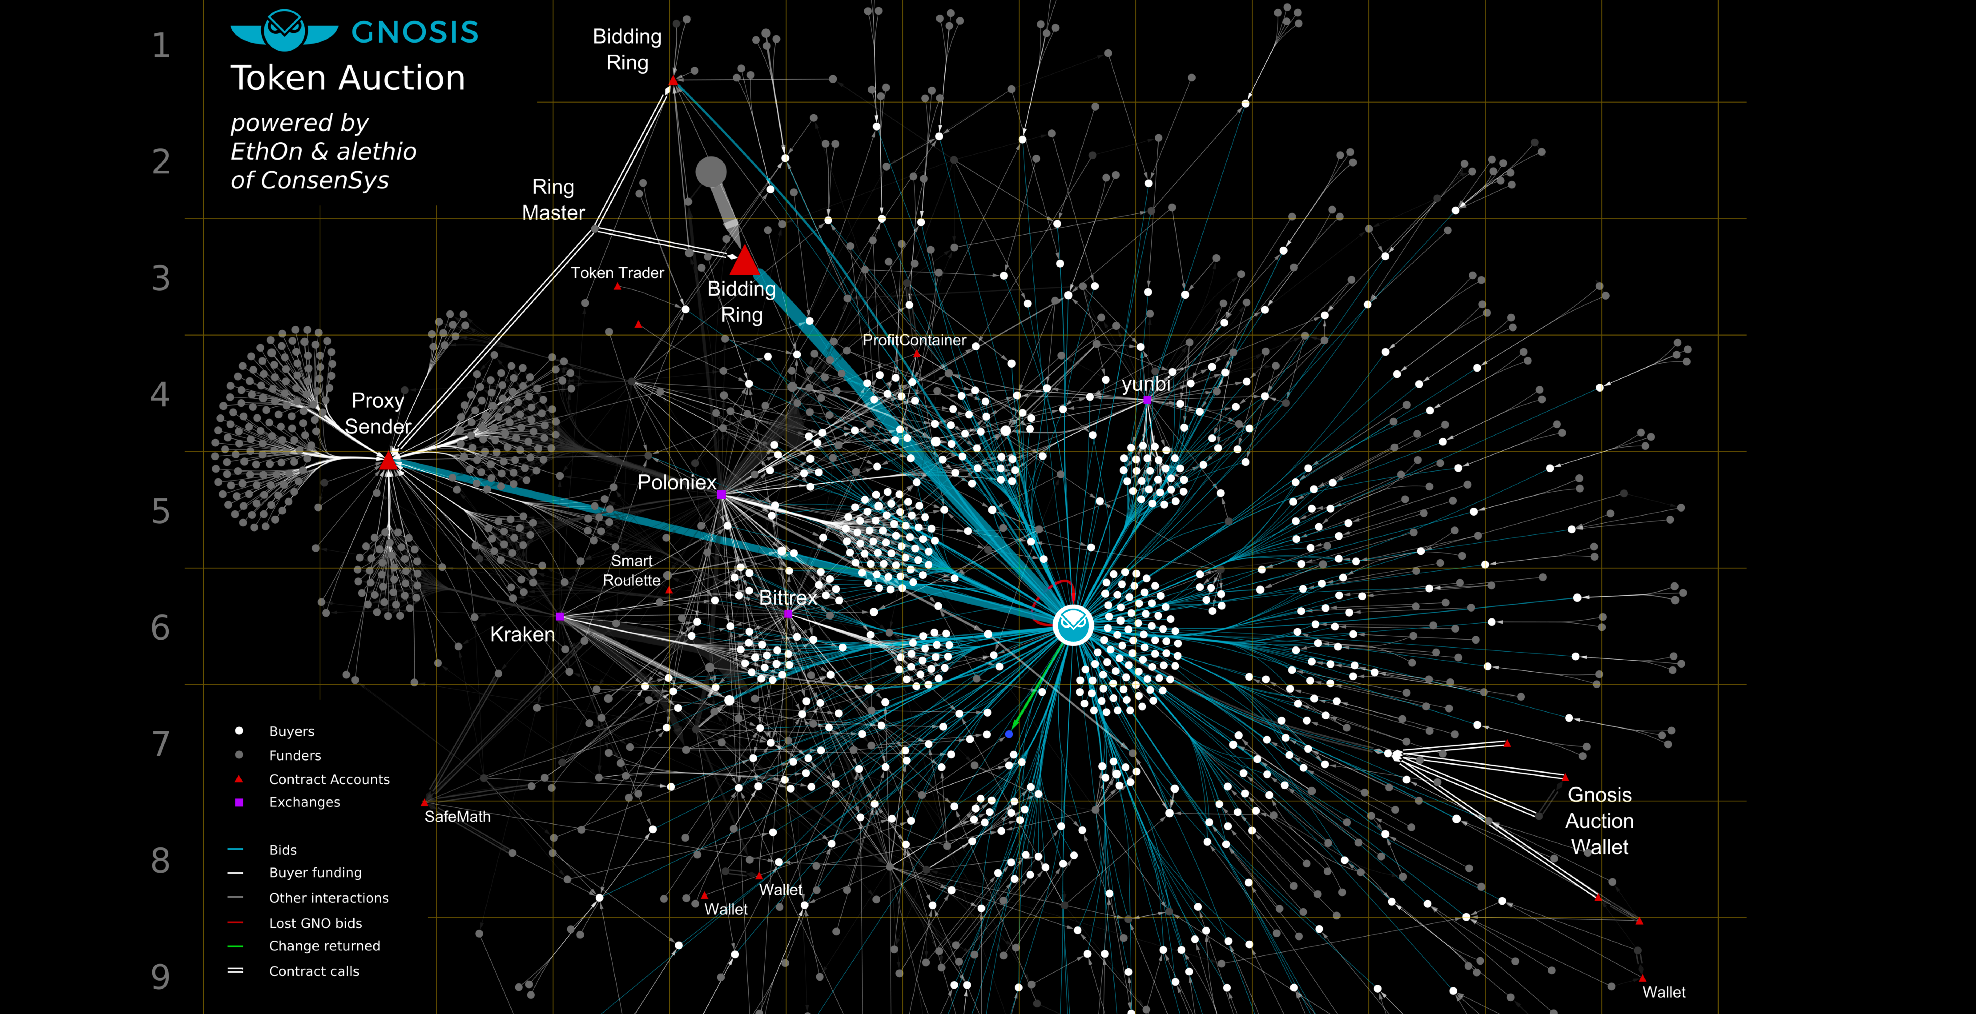
\includegraphics[width=11cm]{../pics/ConsenSys/alethio-tracking-viz}
	\end{figure}
}

\frame{
	\frametitle{Getting paid for your work: The Bounties Network}
	\framesubtitle{\url{https://bounties.network}}
	\begin{figure}
		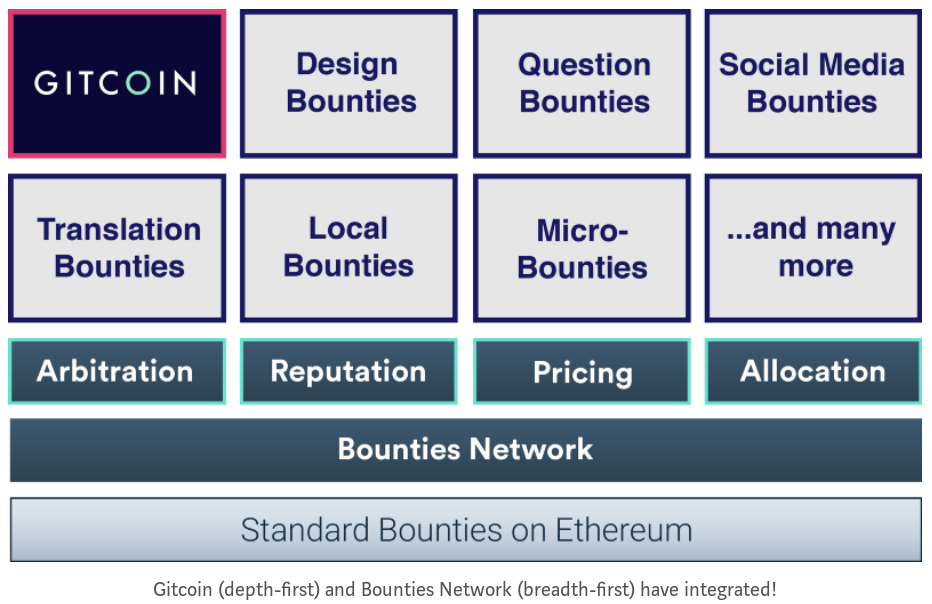
\includegraphics[width=11cm]{../pics/ConsenSys/bounties_network_stack}
	\end{figure}
}

\frame{
	\frametitle{Gitcoin}
	\framesubtitle{\url{https://gitcoin.co}}
	\begin{figure}
		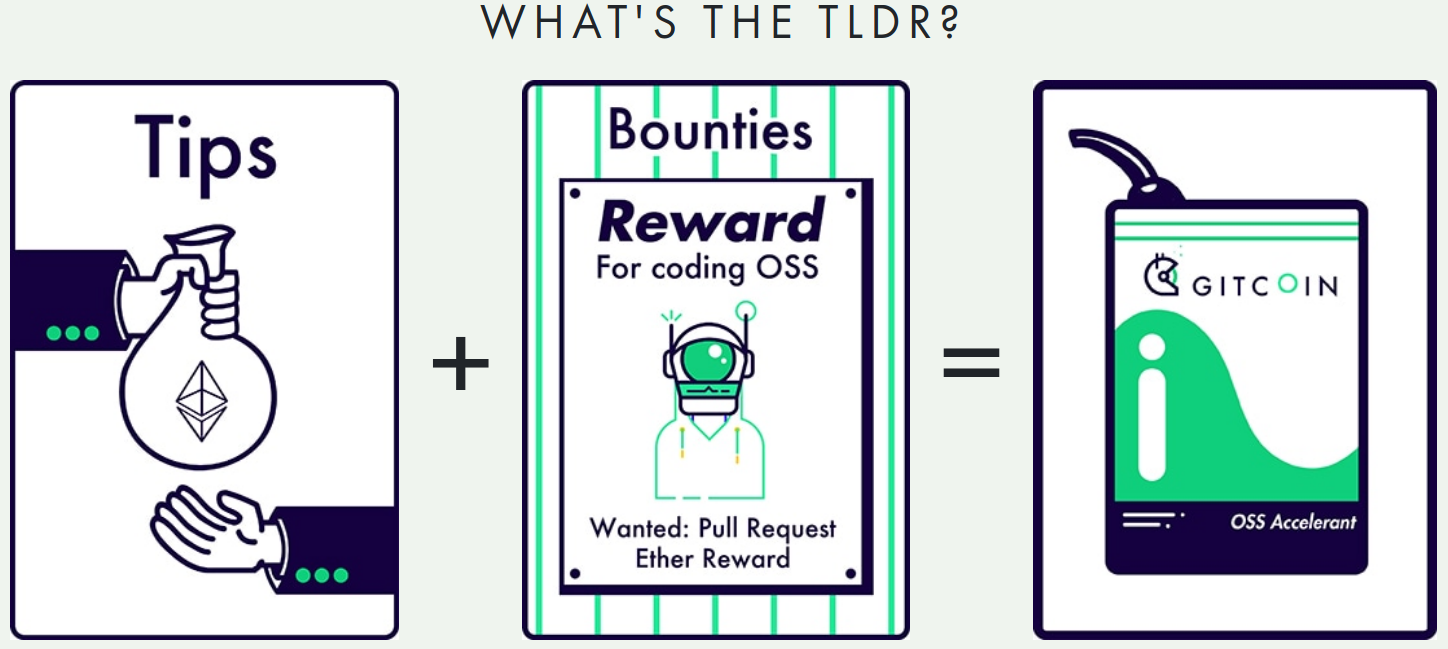
\includegraphics[width=11cm]{../pics/ConsenSys/gitcoin-tldr}
	\end{figure}
}



% ======================================================================================================
%                         Case Studies (ConsenSys) 
% ======================================================================================================
\section{Case Studies}
\frame{
	\frametitle{Transforming Industries}
	%\framesubtitle{}
	\begin{figure}
	
\includegraphics[height=6cm]{../pics/ConsenSys/case_studies/komgo}
	\end{figure}
}

\frame{
	\frametitle{Transforming Industries}
	%\framesubtitle{}
	\begin{figure}
	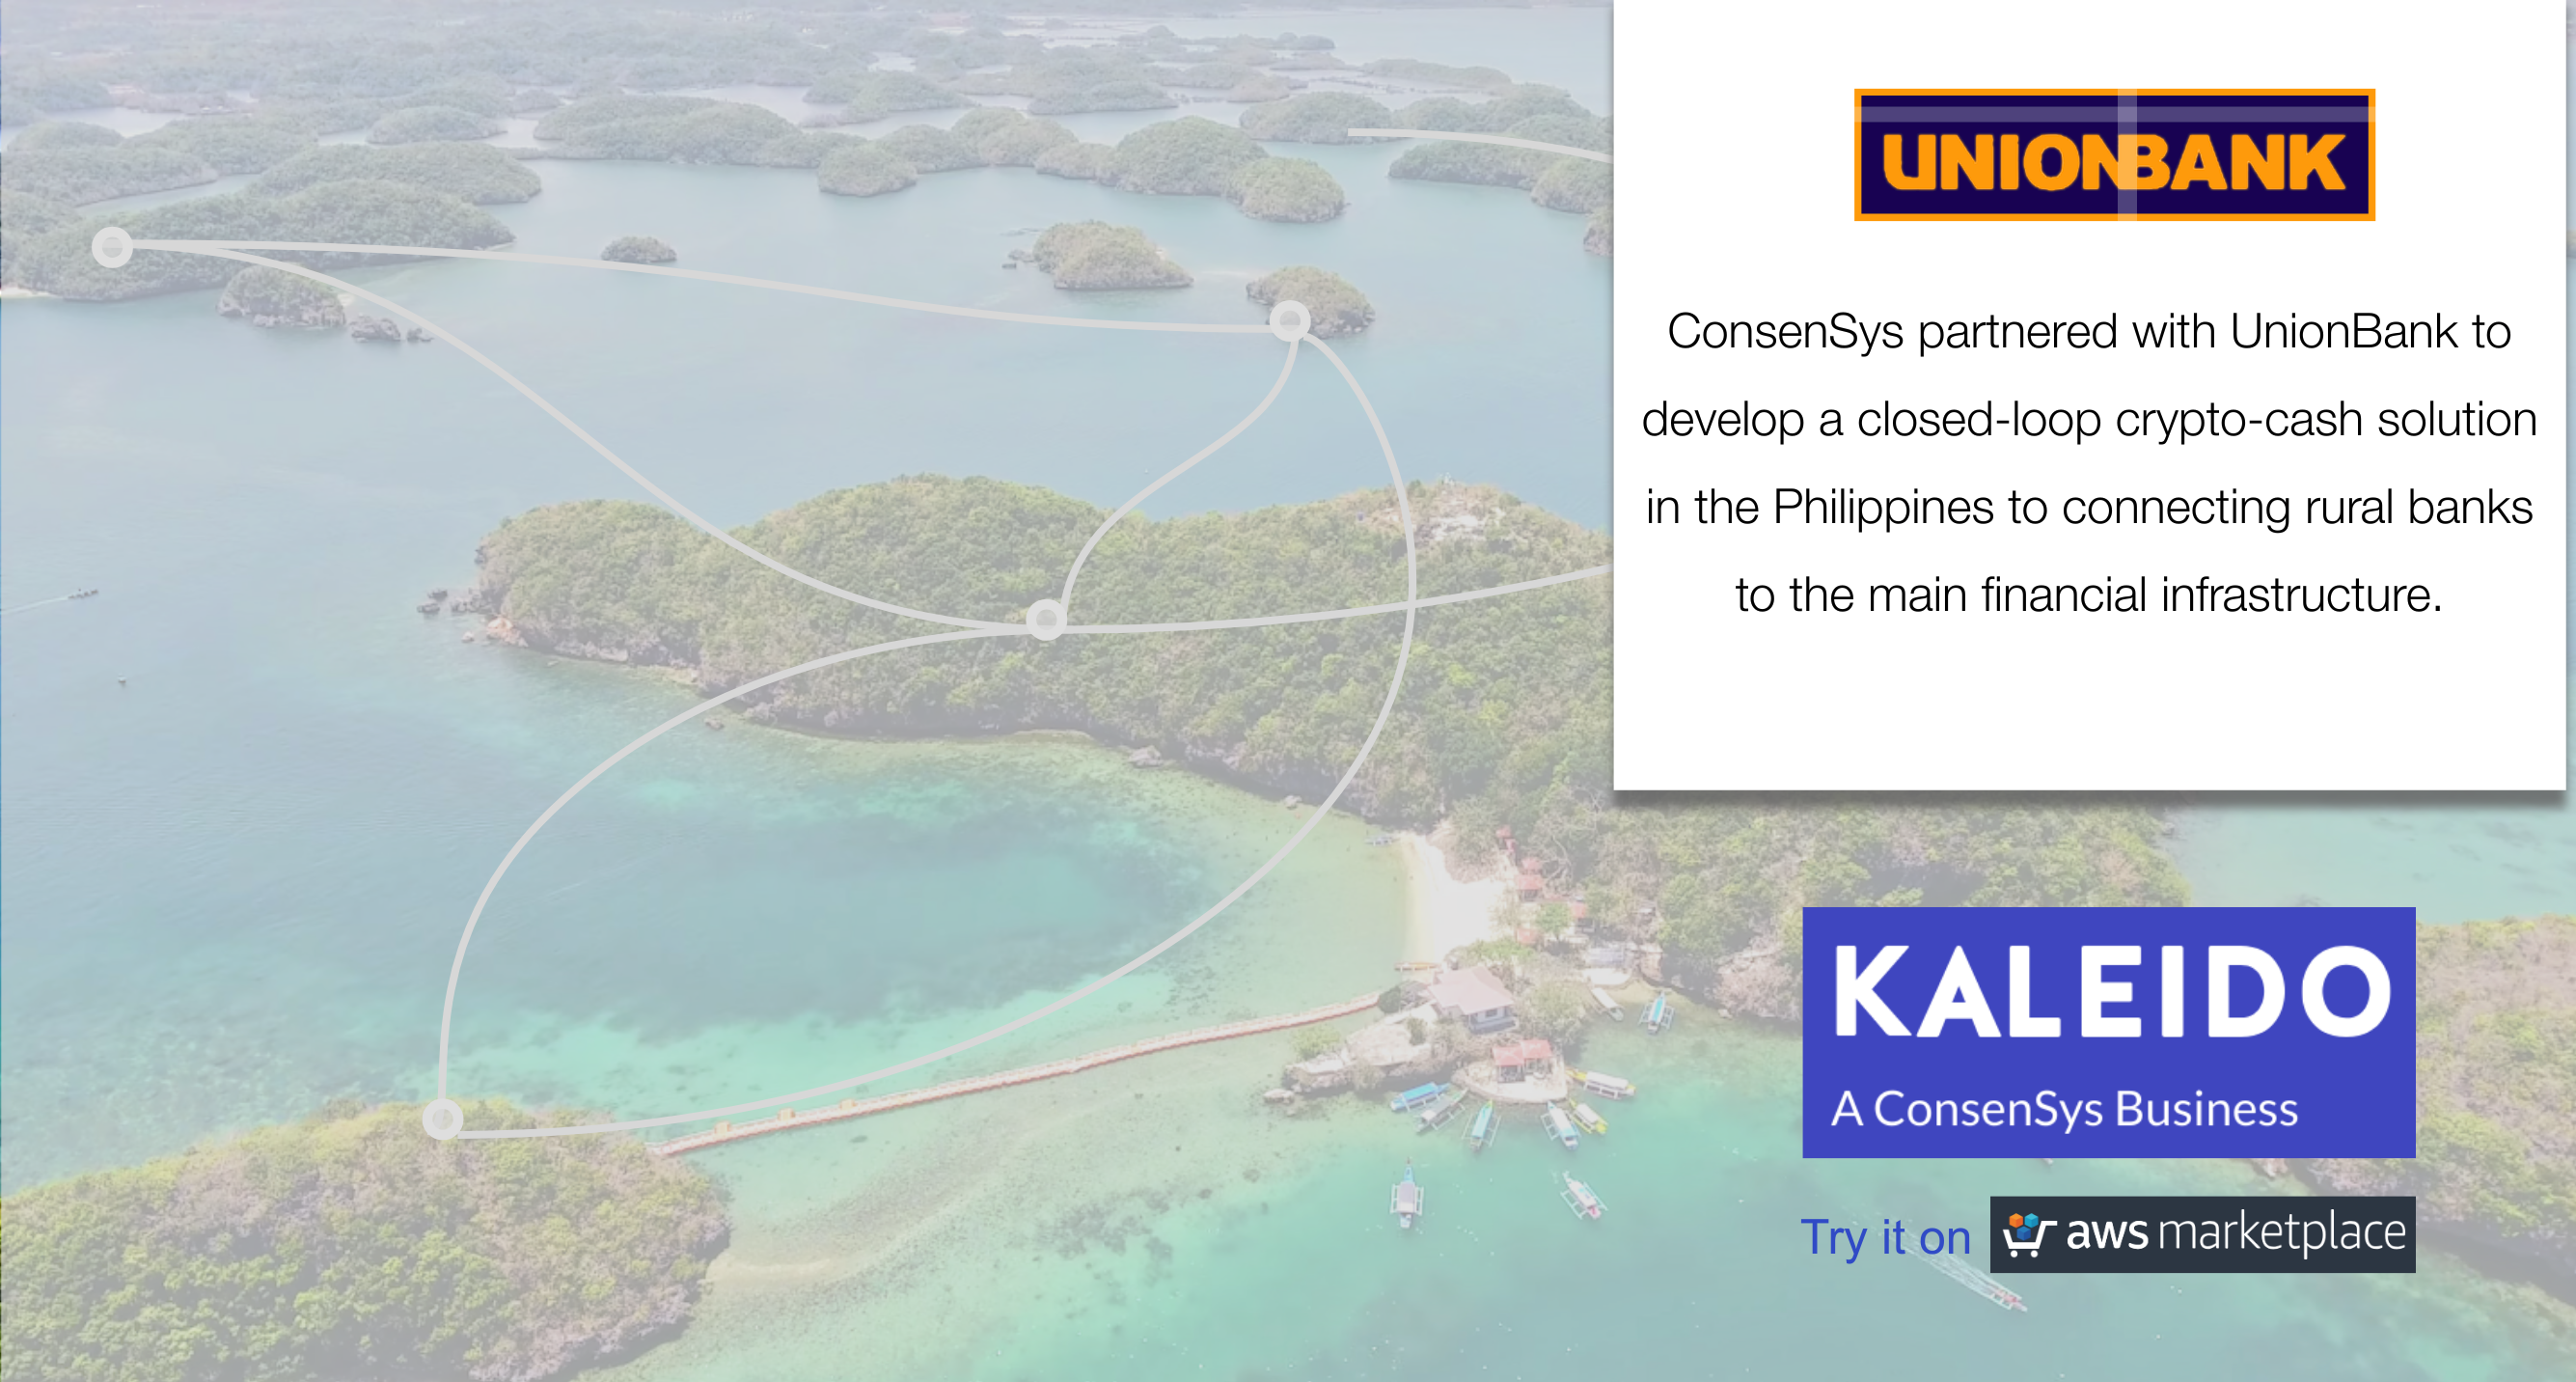
\includegraphics[height=6cm]{../pics/ConsenSys/case_studies/unionbank-kaleido}
	\end{figure}
}

\frame{
	\frametitle{Transforming Industries}
	%\framesubtitle{}
	\begin{figure}
	
\includegraphics[height=6cm]{../pics/ConsenSys/case_studies/mccarthy-tetrault}
	\end{figure}
}


















\frame{
	\centering\Large{Thank you!}\\
	\vspace{2em}
	{\footnotesize
		Email: \href{mailto:marc.lijour@consensys.net}{marc.lijour@consensys.net}\\
		Twitter: \href{https://twitter.com/marclijour}{@marclijour}
	}
}
\frame{
	\frametitle{References}
	% keyword refers to bib file: references-KEYWORD.bib, and to the Tex file: section-KEYWORD.tex  
	\printbibliography 
}
\end{document}

